\documentclass[10pt,a4paper,final]{article} %draft

\usepackage[english, russian]{babel}

\usepackage{geometry}
%\usepackage[a4paper,left=2cm,right=2cm,top=2cm,bottom=2cm,bindingo ffset=0cm]{geometry}

\usepackage[utf8]{inputenc}

\usepackage[final]{pdfpages}

\usepackage{textcomp,enumitem}

\usepackage{amsmath,amsthm,amssymb}

\usepackage{listings}
\usepackage{xcolor}
\usepackage{caption}

\definecolor{codegray}{rgb}{0.95,0.95,0.95}
\definecolor{codepurple}{rgb}{0.58,0,0.82}
\definecolor{codegreen}{rgb}{0,0.5,0} % зеленый цвет
\definecolor{codeblue}{rgb}{0,0,0.5} % синий цвет
\definecolor{codestring}{rgb}{0.64,0.08,0.08} % цвет строк


\lstset{
	language=C++,
	extendedchars=true,
	literate=
	{а}{{\selectfont\char224}}1
	{б}{{\selectfont\char225}}1
	{в}{{\selectfont\char226}}1
	{г}{{\selectfont\char227}}1
	{д}{{\selectfont\char228}}1
	{е}{{\selectfont\char229}}1
	{ж}{{\selectfont\char230}}1
	{з}{{\selectfont\char231}}1
	{и}{{\selectfont\char232}}1
	{й}{{\selectfont\char233}}1
	{к}{{\selectfont\char234}}1
	{л}{{\selectfont\char235}}1
	{м}{{\selectfont\char236}}1
	{н}{{\selectfont\char237}}1
	{о}{{\selectfont\char238}}1
	{п}{{\selectfont\char239}}1
	{р}{{\selectfont\char240}}1
	{с}{{\selectfont\char241}}1
	{т}{{\selectfont\char242}}1
	{у}{{\selectfont\char243}}1
	{ф}{{\selectfont\char244}}1
	{х}{{\selectfont\char245}}1
	{ц}{{\selectfont\char246}}1
	{ч}{{\selectfont\char247}}1
	{ш}{{\selectfont\char248}}1
	{щ}{{\selectfont\char249}}1
	{ъ}{{\selectfont\char250}}1
	{ы}{{\selectfont\char251}}1
	{ь}{{\selectfont\char252}}1
	{э}{{\selectfont\char253}}1
	{ю}{{\selectfont\char254}}1
	{я}{{\selectfont\char255}}1
	{А}{{\selectfont\char192}}1
	{Б}{{\selectfont\char193}}1
	{В}{{\selectfont\char194}}1
	{Г}{{\selectfont\char195}}1
	{Д}{{\selectfont\char196}}1
	{Е}{{\selectfont\char197}}1
	{Ж}{{\selectfont\char198}}1
	{З}{{\selectfont\char199}}1
	{И}{{\selectfont\char200}}1
	{Й}{{\selectfont\char201}}1
	{К}{{\selectfont\char202}}1
	{Л}{{\selectfont\char203}}1
	{М}{{\selectfont\char204}}1
	{Н}{{\selectfont\char205}}1
	{О}{{\selectfont\char206}}1
	{П}{{\selectfont\char207}}1
	{Р}{{\selectfont\char208}}1
	{С}{{\selectfont\char209}}1
	{Т}{{\selectfont\char210}}1
	{У}{{\selectfont\char211}}1
	{Ф}{{\selectfont\char212}}1
	{Х}{{\selectfont\char213}}1
	{Ц}{{\selectfont\char214}}1
	{Ч}{{\selectfont\char215}}1
	{Ш}{{\selectfont\char216}}1
	{Щ}{{\selectfont\char217}}1
	{Ъ}{{\selectfont\char218}}1
	{Ы}{{\selectfont\char219}}1
	{Ь}{{\selectfont\char220}}1
	{Э}{{\selectfont\char221}}1
	{Ю}{{\selectfont\char222}}1
	{Я}{{\selectfont\char223}}1,
	%	{|}{{\textbar}}1,
	%	{||}{{\textbar\textbar}}1
	%	{\&}{{\string&}}1
	%	{==}{{\string==}}1
	%	{\string\\}{{\string\\}}1,
	numbers=left,
	stepnumber=1,
	firstnumber=1,
	numberstyle=\tiny,
	basicstyle=\ttfamily\footnotesize,
	breakatwhitespace=false,
	breaklines=true,
	captionpos=b,
	keepspaces=true,
	showspaces=false,
	showstringspaces=false,
	showtabs=false,
	tabsize=2,
	frame=single,
	keywordstyle=\color{codeblue}, % ключевые слова
	commentstyle=\color{codegreen}, % комментарии
	stringstyle=\color{codestring}, % строки
	%identifierstyle=\color{green}, % стиль для переменных
	backgroundcolor=\color{codegray},
}
%\usepackage{fancyvrb}

%\usepackage{fancyhdr}

%\usepackage{upgreek}

%\usepackage{tipa}

%\usepackage{tikz}

%\usepackage{graphicx}

%\usepackage{pgfplots}

\usepackage{indentfirst}

%\usepackage{gensymb}

%\usepackage{amssymb}

%\usepackage{pdfpages}

\usepackage[unicode, pdftex, colorlinks, urlcolor=blue]{hyperref}

%\usepackage[T2A]{fontenc}


\usepackage{tabularx}
\usepackage{multirow}


\usepackage{graphics}

\linespread{1.5}

\pagestyle{plain}

%\usepackage{listings} 
%\usepackage{moreverb} 

%\setlist[enumerate,itemize]{leftmargin=1.2cm} %отступ в перечислениях

\hypersetup{
	colorlinks=true,
	linkcolor=black,
	%allcolors=[RGB]{0 0 0}}
	}
	%\lstloadlanguages{ [LaTeX] TeX}
	
	\lstloadlanguages{ [LaTeX] TeX}
	
	
	
	\textheight=24cm 
	\textwidth=16cm
	\oddsidemargin=0pt 
	\topmargin=-1.5cm
	\parindent=24pt 
	\parskip=0pt 
	\tolerance=2000 
	\flushbottom 
	
	%\usepackage[font=scriptsize]{caption}
	\usepackage[labelsep=period]{caption}
	
	\begin{document}
\thispagestyle{empty}

\begin{center}
	{\Large МИНОБРНАУКИ РОССИИ}\\
	~\\
	{\large ФЕДЕРАЛЬНОЕ ГОСУДАРСТВЕННОЕ БЮДЖЕТНОЕ ОБРАЗОВАТЕЛЬНОЕ УЧРЕЖДЕНИЕ ВЫСШЕГО ПРОФЕССИОНАЛЬНОГО ОБРАЗОВАНИЯ}\\
	~\\
	{\Large \bf <<САНКТ-ПЕТЕРБУРГСКИЙ ПОЛИТЕХНИЧЕСКИЙ УНИВЕРСИТЕТ ПЕТРА ВЕЛИКОГО>>}\\
	~\\
	{\large Институт компьютерных наук и кибербезопасности}\\
	{\large Высшая школа технологий искусственного интеллекта}\\
	{\large Направление 02.03.01 Математика и компьютерные науки}\\
	~\\
	~\\
	~\\
	~\\
	{\Large \bf Отчет о выполнении лабораторной работы №6}\\
	{\Large по дисциплине <<Теория графов>> }\\
	~\\
	~\\
	
	{\Large  Построение словаря на основе хеш-таблицы и В+-дерева}\\
	%	{\Large \bf }\\ 	
	
	~\\
	~\\
	~\\
	~\\
	~\\
	~\\
	~\\
	{\large Обучающийся: \underline{\hspace{3.5cm}} \qquad\qquad Гладков И.А.}\\
	~\\
	{\large Руководитель: \underline{\hspace{3.5cm}} \hspace{16mm} Востров А.В.}\\
	~\\
	~\\
\end{center}
\begin{flushright}
	
	«\underline{\hspace{1cm}}»\underline{\hspace{3cm}}20\underline{\hspace{0.7cm}}г.
\end{flushright}
~\\
\begin{center}
	{\large Санкт-Петербург, 2024}
\end{center}
\newpage

\tableofcontents

\newpage


\section* {Введение}
\addcontentsline{toc}{section}{Введение}
\par В данной работе необходимо разработать словарь, в котором будут присутствовать операции добавления, удаления, поиска, очистки словаря и  дополнение слов из текстового файла. Для хранения данных необходимо использовать хэш-таблица и B+ дерево. 

%\par Работа была выполнена в среде Visual Studio 2022 на языке программирования С++.


\newpage
\section{Математическое описание}
\subsection{Определение хеш-функции}

Хеш-функция — это математическая функция, которая преобразует значение ключа (входные данные произвольного размера) в фиксированное значение, называемое \textbf{хешем} или \textbf{хеш-значением}. Это значение служит для идентификации ключа в структуре данных, чаще всего в хеш-таблицах, или для вычисления адреса хранения данных в памяти или на диске. Основная цель хеш-функции — быстро и эффективно определить место хранения записи по ключу, так как хеш-значение указывает на конкретный адрес (индекс массива, кластер на диске или другой элемент структуры).

Хеш-функция разрабатывается таким образом, чтобы минимизировать вероятность того, что два разных ключа будут иметь одинаковое хеш-значение, но, поскольку мощность множества ключей зачастую значительно больше размера пространства возможных хешей, в большинстве случаев возникает ситуация, когда два или более разных ключа будут иметь одинаковое хеш-значение. Это явление называется \textit{коллизией}.

Важное требование к хеш-функции — равномерное распределение ключей по множеству возможных хеш-значений. При этом множество возможных ключей обычно гораздо больше, чем размер пространства хеш-значений, что делает возникновение коллизий неизбежным. 

\subsection{Хеш-функция}

В данной работе в качестве хеш-функции использовалось выражение $S = \sum_{i=0}^{n}(7+i)x_{i}^{i}$, где $n$ -- количество букв в слове; $x_i$ -- код $i$-ого символа слова по таблице ASCII. Выражение хешируется как:

\[
H(S) = (7 \cdot x_0^{0} + 8 \cdot x_1^{1} + 9\cdot x_2^{2} +  \ldots  + (7+n) \cdot  x_n^n) \mod m 
\]

где:
\begin{itemize}
	\item $x_i$ — код по таблице ASCII $i$-го символа слова,
	\item $n$ — количество символов в слове,
	\item $m$ — размер хеш-таблицы или общее количество бакетов.
\end{itemize}


\subsection{Хеш-таблица}

\textbf{Хеш-таблица} — это структура данных, которая представляет собой одну из реализаций ассоциативной памяти. Она используется для хранения пар вида \texttt{(ключ, значение)} и поддерживает три основные операции: добавление пары, поиск и удаление пары по ключу.

Хеш-таблицы бывают двух основных типов: с открытой адресацией и с использованием метода цепочек (списков). В хеш-таблице с открытой адресацией каждый элемент массива либо содержит пару \texttt{(ключ, значение)}, либо пуст, тогда как в хеш-таблице с цепочками каждый элемент является списком пар, что позволяет хранить несколько пар в одном месте массива. Массив хеш-таблицы состоит из $n$ ячеек, каждая из которых в зависимости от типа может содержать пару или список пар.

Ключевая часть работы хеш-таблицы — это \textbf{хеш-функция}, которая преобразует ключ в индекс массива хеш-таблицы. Важной особенностью является то, что хеш-функция зависит только от ключа и не использует значение. Впрочем, как было указано ранее (см. раздел 1.2), возможны ситуации, при которых различные ключи могут иметь одинаковый хеш — это явление называется \textbf{коллизией}. Для разрешения коллизий используются различные стратегии, такие как линейное пробирование при открытой адресации или хранение нескольких элементов в одной ячейке с помощью списка в методе цепочек.

Одним из важнейших параметров хеш-таблицы является \textbf{коэффициент загрузки}, который равен отношению числа хранимых элементов к количеству ячеек в массиве хеш-таблицы. Этот параметр оказывает значительное влияние на эффективность операций: чем выше коэффициент загрузки, тем больше вероятность коллизий, что может замедлить работу таблицы.

В идеальных условиях, при правильно подобранной хеш-функции и разумном значении коэффициента загрузки, все три основные операции (добавление, поиск и удаление) могут выполняться за время $O(1)$ в среднем. Однако в худшем случае время выполнения может быть значительно больше, особенно если происходит много коллизий. Когда коэффициент загрузки превышает определённый порог, возникает необходимость в \textbf{рехешировании} — процессе, при котором создаётся новый массив большего размера, и все существующие пары из старого массива переносятся в новый, с пересчётом индексов на основе новой хеш-функции.\\
Структура реализованной хеш-таблицы представлена \hyperref[fig:hash]{риcунке 1}

\begin{figure}[htbp]
	\centering
	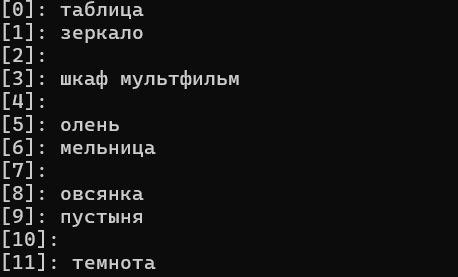
\includegraphics[width=0.5\linewidth]{hash}
	\caption{Реализованная структура хеш-таблицы}
	\label{fig:hash}
\end{figure}



\subsubsection{Разрешение коллизий методом цепочек}

Метод цепочек, или списков, является популярным способом разрешения коллизий в хеш-таблицах. В этом методе каждый элемент массива хеш-таблицы представляет собой связанный список пар \texttt{(ключ, значение)}. Когда несколько ключей хешируются в одно и то же значение (то есть происходит коллизия), все соответствующие пары помещаются в один и тот же список или массив (бакет). 

Когда в методе цепочек при добавлении новой пары возникает коллизия, эта пара добавляется в конец массива (списка), связанного с индексом, на который указала хеш-функция. Время добавления элемента в конец массива составляет $O(n)$, где $n$ — длина массива.

Операции удаления и поиска элемента в массиве  требуют последовательного прохода по нему. Время поиска или удаления элемента будет $O(n)$, где $n$ — количество элементов в массиве. 


Среднее время выполнения операций в хеш-таблице зависит от \textbf{коэффициента загрузки} $\alpha$, который равен отношению количества хранимых элементов к количеству бакетов. Если распределение хешей равномерное, то средняя длина массива при каждом индексе будет небольшой, и время поиска элемента составит $O(1 + \alpha)$. При низком коэффициенте загрузки ($\alpha \ll 1$) время выполнения операций близко к $O(1)$. Однако при высоком коэффициенте загрузки ($\alpha \gg 1$) длина массивов увеличивается, что замедляет операции поиска и удаления, делая их время выполнения ближе к $O(n)$.

\textbf{Операции с массивом}:
\begin{itemize}
	\item \textbf{Добавление элемента}: Элемент добавляется в конец массива. Сложность операции — $O(n)$, где $n$ — количество элементов в массиве. 
	\item \textbf{Удаление элемента}: Требуется найти элемент, после чего удалить его. Сложность операции — $O(n)$.
	\item \textbf{Поиск элемента}: Необходимо последовательно пройти по массиву и найти элемент. Сложность операции — $O(n)$.
%	\item \textbf{Подсчёт элементов по условию} (count): Проход по списку с проверкой каждого элемента на заданное условие. Сложность операции — $O(n)$.
\end{itemize}



\subsection{B+-дерево}
\textbf{B+-дерево} — это сбалансированная и сильно ветвистая структура данных, предназначенная для эффективного хранения и поиска элементов. Основное преимущество B+-дерева — это возможность выполнения операций поиска, добавления и удаления за $O(\log n)$, где $n$ — количество элементов в дереве.

\textbf{Сбалансированность} означает, что длина путей от корня до любого листа одинакова, что предотвращает деградацию производительности. \textbf{Ветвистость} дерева подразумевает, что каждый узел содержит ссылки на множество потомков, что уменьшает глубину дерева и, следовательно, время выполнения операций.

B+-дерево степени $t > 2$ обладает следующими основными свойствами:
\begin{itemize}
	\item Каждый узел содержит хотя бы один ключ, при этом ключи в узлах упорядочены по возрастанию. Корневой узел содержит от 1 до $2t - 1$ ключей, а все остальные узлы содержат от $t - 1$ до $2t - 1$ ключей.
	\item Листовые узлы не имеют потомков. Внутренние узлы, содержащие $n$ ключей $K_1, K_2, ..., K_n$, имеют $n + 1$ потомков. При этом:
	\begin{itemize}
		\item Первый потомок и все его ключи меньше $K_1$.
		\item Потомки между $K_{i-1}$ и $K_i$ содержат ключи, принадлежащие интервалу $(K_{i-1}, K_i)$ для $2 \leq i \leq n$.
		\item Последний потомок и все его ключи больше $K_n$.
	\end{itemize}
	\item Все листовые узлы находятся на одном уровне, что гарантирует равномерную глубину.
	\item Листовые узлы содержат указатели на своих соседей, что обеспечивает эффективный обход дерева в порядке возрастания ключей.
\end{itemize}

\subsection{Операции над B+-деревом}
\subsubsection{Поиск}
Поиск элемента в B+-дереве начинается с корня и продолжается до листа. Благодаря свойству, что каждый потомок имеет ключи из определённого интервала, можно эффективно направлять поиск. Пусть требуется найти ключ $k$. В каждом внутреннем узле производится одно из следующих действий:
\begin{itemize}
	\item Если $k$ меньше наименьшего ключа узла, спускаемся к первому потомку.
	\item Иначе находим ключи $K_i$, при которых выполняется $K_i \leq k < K_{i+1}$, и спускаемся к $i+1$-му потомку.
	\item Если $k \geq K_n$, спускаемся к последнему потомку.
\end{itemize}
Процесс продолжается до тех пор, пока не будет найден соответствующий лист, который либо содержит ключ $k$, либо указывает на его отсутствие. Поскольку дерево сбалансировано, глубина поиска составляет $O(\log n)$.

\subsubsection{Добавление}
Чтобы добавить новый элемент в B+-дерево, сначала необходимо найти подходящий листовой узел для вставки ключа. Алгоритм добавления следующий:
\begin{itemize}
	\item Если узел не заполнен, то ключ просто добавляется, сохраняя порядок. 
	\item Если узел заполнен (содержит $2t - 1$ ключей), происходит расщепление:
	\begin{itemize}
		\item Узел делится на два, при этом половина ключей переносится в новый узел.
		\item Копия наименьшего ключа из нового узла добавляется в родительский узел.
		\item Если родительский узел также заполнен, процесс расщепления продолжается вверх по дереву.
	\end{itemize}
	\item Если расщепляется корневой узел, создаётся новый корень, содержащий один ключ и две ссылки на потомков.
\end{itemize}
Добавление элемента требует $O(\log n)$ операций, поскольку в худшем случае может потребоваться проход от листа до корня.

\subsubsection{Удаление}
Алгоритм удаления элемента из B+-дерева также начинается с поиска соответствующего листового узла. После нахождения ключа выполняются следующие шаги:
\begin{itemize}
	\item Если после удаления узел остаётся наполовину заполненным (содержит не менее $t - 1$ ключей), операция завершается.
	\item Если узел становится менее чем наполовину заполненным, необходимо перераспределить ключи с соседними узлами. Можно взять ключ у левого или правого «брата» (соседа на том же уровне).
	\item Если перераспределение невозможно, узлы объединяются с соседом, и ключ, указывающий на объединённые узлы, удаляется из родительского узла.
\end{itemize}
Удаление также выполняется за $O(\log n)$, так как может потребоваться корректировка структуры вплоть до корня.

\subsubsection{Пример Б+-дерева}
На \hyperref[fig:pic2]{риcунке 2} представлен пример структуры Б+-дерева. 

\begin{figure}[htbp]
	\centering
	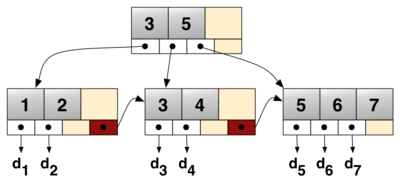
\includegraphics[width=0.7\linewidth]{pic2.png}
	\caption{Пример структуры Б+-дерева}
	\label{fig:pic2}
\end{figure}
\newpage

На \hyperref[fig:tree]{рисунках 3-4} представлена реализованная заполненная структура Б+-дерева.

\begin{figure}[htbp]
	\centering
	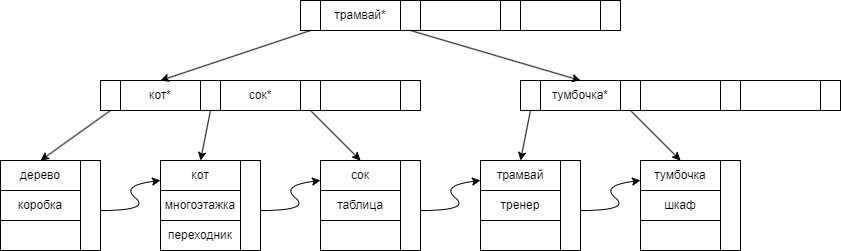
\includegraphics[width=1.05\linewidth]{tree.png}
	\caption{Пример реализованной заполненной структуры Б+-дерева}
	\label{fig:tree}
\end{figure}

\begin{figure}[htbp]
	\centering
	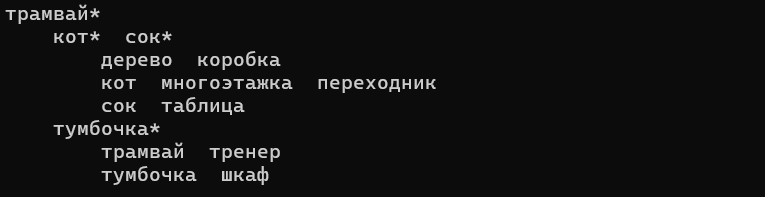
\includegraphics[width=1.1\linewidth]{tr.png}
	\caption{Пример реализованной заполненной структуры Б+-дерева}
	\label{fig:tr}
\end{figure}




\newpage
\section{Особенности реализации}

\subsection{Класс HashTable}
 Класс HashTable представляет из себя реализацию хеш-таблицы. В нем существуют следующие перменные:
 \begin{enumerate}
 	
 	\item \textbf{int count\_backets} -- количество бакетов в хеш-таблице;
 	\item \textbf{int count\_words} -- количество слов в хеш-таблице;
 	\item \textbf{vector<vector<string>> backets} -- динамический массив бакетов; в каждом бакете динамический массив, хранящий в себе слова;
 	\item \textbf{vector<string> conj} -- массив, хранящий в себе слова, которые не добавляются в хеш-таблицу (местоимения, союзы и тп.);
 	\item \textbf{double percent} -- коэффициент заполнения таблицы;
 	
 \end{enumerate}


\subsubsection{Метод HashCode}
Вход: \texttt{string str} - слово, добавляемое в хеш-таблицу. 

Выход: \texttt{int} - хеш слова. \\

\par Метод \texttt{hashFunction} вычисляет хеш-значение для слова \texttt{str}. Данный метод служит для вычисления хеша, которое затем используется для определения индекса в хеш-таблице.

\par Алгоритм работы следующий: метод инициализирует переменную \texttt{result} значением \texttt{indx}, которое установлено равным 7. Далее для каждого символа строки метод вычисляет числовое значение символа \texttt{x} и последовательно умножает его на себя (возводя в степень, равную индексу символа в строке). Итоговое значение для каждого символа добавляется к \texttt{result} с учетом текущего индекса символа и базового значения \texttt{indx}.

Код метода представлен в листинге 1. \begin{lstlisting}[label=hashCodeExample, caption = Метод HashCode] 
int HashTable::HashCode(string str) {	
	int result = 0;
	int indx = 7;
	
	result = indx;
	
	for (int i = 1; i < str.size() + 1; i++) {
		int x = static_cast<int>(str[i - 1]);
		for (int j = 1; j < i; j++) {
			x *= x;
		}
		result += (indx + i) * x;
	}
	return result;
} \end{lstlisting}


\subsubsection{Метод Contains}
Вход: string str — слово для поиска.

Выход: bool — \texttt{true}, если слово найдено, иначе \texttt{false}. 

\par Метод \texttt{Contains} проверяет, содержится ли слово \texttt{str} в хеш-таблице. Для этого вычисляется хеш-код слова, определяется соответствующий бакет, и производится поиск слова в этом бакете. Если слово найдено, возвращается \texttt{true}, в противном случае — \texttt{false}.

Код метода представлен в листинге 2. \begin{lstlisting}[label=containsMethod, caption = Метод Contains] 
	bool HashTable::Contains(string str) {
		int code = HashCode(str);
		int n = code % count_backets;
		n = n < 0 ? -1 * n : n;
		for (string word : backets[n]) {
			if (word == str)
			return true;
		}
		return false;
	} \end{lstlisting}


\subsubsection{Метод Add}
Вход: string str — строка для добавления. \par
Выход: слово добавлено в словарь. \par
\par Метод \texttt{Add} добавляет строку \texttt{str} в хеш-таблицу. Если строка уже существует в таблице, она не добавляется. При превышении заполненности таблицы на 75% происходит расширение количества бакетов в два раза с перераспределением элементов.

Код метода представлен в листинге 3. \begin{lstlisting}[label=addMethod, caption = Метод Add]
	void HashTable::Add(string str) {
		str = toDown(str);
		if (!Contains(str)) {
			if (percent >= 75) {
				vector<vector<string>> buf(count_backets * 2);
				count_backets *= 2;
				for (vector<string> strings : backets) {
					for (string s : strings) {
						int code = HashCode(s);
						int n = code % count_backets;
						n = n < 0 ? -1 * n : n;
						buf[n].push_back(s);
					}
					
				}
				backets = buf;
			}
			int code = HashCode(str);
			int n = code % count_backets;
			n = n < 0 ? -1 * n : n;
			backets[n].push_back(str);
			count_words++;
			percent = static_cast<double>(count_words) / count_backets * 100;
		}
	} \end{lstlisting}



\subsubsection{Метод Delete}
Вход: string str — слово для удаления. \par
Выход: слово удалено из словаря. \par
\par Метод \texttt{Delete} удаляет слово \texttt{str} из хеш-таблицы, если оно там содержится. Сначала проверяется наличие слова в таблице, после чего оно удаляется из соответствующего бакета.

Код метода представлен в листинге 4. \begin{lstlisting}[label=deleteMethod, caption = Метод Delete] 
void HashTable::Delete(string str) {
	str = toDown(str);
	if (Contains(str)) {
		int code = HashCode(str);
		int n = code % count_backets;
		n = n < 0 ? -1 * n : n;
		for (int i = 0; i < backets[n].size(); i++) {
			if (backets[n][i] == str) {
				backets[n].erase(backets[n].begin() + i);
				count_words--;
				break;
			}
		}
	}
} \end{lstlisting}


\subsubsection{Метод toDown}
Вход: string str — слово для преобразования. \par
Выход: слово, преобразованное в нижний регистр. \par
\par Метод \texttt{toDown} преобразует все буквы слова \texttt{str} в нижний регистр, поддерживая как латинские, так и кириллические символы.

Код метода представлен в листинге 5. \begin{lstlisting}[label=toDownMethod, caption = Метод toDown] 
	 string HashTable::toDown(string str) {
	 	string result = "";
	 	for (char c : str) {
	 		if (c >= 'A' && c <= 'Z') {
	 			c = c + ('a' - 'A');
	 		}
	 		if (c >= 'А' && c <= 'Я') {
	 			c = c + ('а' - 'А');
	 		}
	 		result += c;
	 	}
	 	return result;
	 }\end{lstlisting}
 
 
 \subsubsection{Метод is\_a\_conj}
 Вход: string str — слово для проверки. \par
 Выход: bool — \texttt{true}, если слово является исключением, \texttt{false} — если нет. \par
 \par Метод \texttt{is\_a\_conj} проверяет, является ли слово \texttt{str} словом-исключением, сравнивая его с перечнем слов-исключений \texttt{conj}.
 
 Код метода представлен в листинге 6. \begin{lstlisting}[label=isAConjMethod, caption = Метод is\_a\_conj] 
 
 bool HashTable::is_a_conj(string str) {
 	str = toDown(str);
 	for (string word : conj) {
 		if (str == word) {
 			return true;
 		}
 	}
 	return false;
 } \end{lstlisting}


\subsubsection{Метод Delete\_all}
Вход: хеш-таблица. \par
Выход: словарь полностью очищен. \par
\par Метод \texttt{Delete\_all} полностью очищает хеш-таблицу, сбрасывая все бакеты, количество слов и восстанавливая исходное количество бакетов.

Код метода представлен в листинге 7. \begin{lstlisting}[label=deleteAllMethod, caption = Метод Delete\_all]
void HashTable::Delete_all() {
	vector<vector<string>> buf(6);
	backets = buf;
	count_backets = 6;
	count_words = 0;
} \end{lstlisting}



\subsubsection{Метод From\_file}
Вход: string str — путь к файлу. \par
Выход: слова из файла добавлены в словарь. \par
\par Метод \texttt{From\_file} считывает слова из файла по указанному пути \texttt{str}, очищает их от знаков пунктуации и добавляет в хеш-таблицу. Исключения не добавляются. В случае неудачной попытки открытия файла выводится сообщение об ошибке.

Код метода представлен в листинге 8. \begin{lstlisting}[label=fromFileMethod, caption = Метод From\_file]
void HashTable::From_file(string str) {
	//std::filesystem::path file_path = str;
	//ifstream file(R"(str)");
	ifstream file(str);
	if (!file.is_open()) {
		printf("\nНе удалось открыть файл\n\n");
	}
	else {
		string line;
		vector<string> words = { "" };
		int last_index = 0;
		char c;
		int k = 0;
		while (file.get(c)) {
			if (c != ',' && c != '.' && c != ':' && c != ';' && c != '!' && c != '?' && c != '-' && c != '?'
			&& c != '(' && c != ')' && c != '{' && c != '}' && c != '[' && c != ']' && c != '\''
			&& c != '"') {
				if (c != ' ' && c != '\n') {
					words[last_index] += c;
				}
				else {
					if (words[last_index].size() > 0) {
						words.push_back("");
						last_index++;
					}
				}
			}
			
		}
		
		if (words[words.size() - 1] == "") {
			words.pop_back();
		}
		
		file.close();
		for (auto word : words) {
			if (!this->is_a_conj(word)) {
				this->Add(word);
			}
		}
		
		printf("\nСлова из файла добавлены в словарь\n\n");
	}
}\end{lstlisting}


\subsubsection{Метод menu}
Вход: создание консольного меню, для работы с хеш-таблицей. \par
Выход: консольное меню для работы с хеш-таблицей. \par
\par Метод \texttt{menu} реализует цикл пользовательского меню, предоставляя различные опции для работы со словарём, такие как просмотр содержимого, добавление и удаление слов, очистка словаря, проверка наличия слов, загрузка данных из файла и просмотр списка исключений. Меню завершает свою работу при выборе пункта выхода.

Код метода представлен в листинге 9. \begin{lstlisting}[label=menuMethod, caption = Метод menu] 
void HashTable::menu() {
	while (true) {
		printf("\n--------------------- Словарь (хэш-таблица)---------------------\n");
		printf("Выберите действие:\n");
		printf("[1] - просмотр содержимое словаря \n");
		printf("[2] - добавление нового слова\n");
		printf("[3] - удаление слова\n");
		printf("[4] - проверка наличие слов в словаре\n");
		printf("[5] - полная очистка словаря\n");
		printf("[6] - добавление слов из файла\n");
		printf("[7] - просмотр список недобавляющихся слов\n");
		
		printf("[0] - выход из словаря\n");
		printf("---------------------------------------------------\n");
		
		int choose;
		bool out = false;
		string word;
		string file;
		vector<string> files = { "Мастер и Маргарита.txt", "Преступление и наказание.txt" };
		int k;
		bool flag_out_path;
		
		while (true) {
			
			cin >> choose;
			
			// Проверка на корректность ввода
			if (std::cin.fail()) {
				std::cin.clear(); // Сброс состояния потока
				std::cin.ignore(std::numeric_limits<std::streamsize>::max(), '\n'); // Очистка буфера ввода
				std::cout << "Некорректный ввод! Пожалуйста, введите число." << std::endl;
			}
			else if (choose < 0 || choose > 7) {
				// Проверка, что число находится в нужном диапазоне
				std::cout << "Число вне диапазона! Пожалуйста, введите число от 0 до 7."<< std::endl;
			}
			else {
				break; // Выход из цикла, если ввод корректен и число в диапазоне
			}
		}
		
		
		switch (choose)
		{
			case 0:
			out = true;
			break;
			case 1:
			if (count_words == 0) {
				printf("\nСловарь пуст\n\n");
			}
			else {
				printf("\nСодержимое словаря:\n");
				printf("[1] - по бакетам \n");
				printf("[2] - списком \n\n");
				printf("Как вы хотите? Введите свой выбор: ");
				while (true) {
					
					cin >> k;
					
					// Проверка на корректность ввода
					if (std::cin.fail()) {
						std::cin.clear(); // Сброс состояния потока
						std::cin.ignore(std::numeric_limits<std::streamsize>::max(), '\n'); // Очистка буфера ввода
						std::cout << "Некорректный ввод! Пожалуйста, введите число." << std::endl;
					}
					else if (k < 1 || k > 2) {
						// Проверка, что число находится в нужном диапазоне
						std::cout << "Число вне диапазона! Пожалуйста, введите число от 1 до 2." << std::endl;
					}
					else {
						break; // Выход из цикла, если ввод корректен и число в диапазоне
					}
				}
				
				
				switch (k) {
					case 2:
					k = 1;
					for (auto words : backets) {
						for (auto word : words) {
							printf("%d. %s \n", k, word.c_str());
							k++;
						}
					}
					
					break;
					
					case 1:
					k = 0;
					for (auto words : backets) {
						printf("[%d]: ", k);
						for (auto word : words) {
							cout << word << ' ';
						}
						cout << endl;
						k++;
					}
					printf("\nКоличество слов: %d\n\n", count_words);
					break;
				}
			}
			break;
			case 2:
			while (true) {
				printf("Введите слово для добавления в словарь (для выхода в меню напишите '0'): ");
				cin >> word;
				if (word == "0") {
					break;
				}
				else {
					if (!Contains(word)) {
						if (!is_a_conj(word)) {
							this->Add(word);
							printf("\n\tСлово '%s' добавлено в словарь\n\n", word.c_str());
							//break;
						}
						else {
							printf("\n\tСлово '%s' не добавлено в словарь, так как оно входит в список недобавляющихся слов :(\n\n", word.c_str());
						}
					}
					else {
						printf("\n\tСлово '%s' не добавлено в словарь, оно уже там присутсвует\n\n", word.c_str());
					}
				}
				
			};
			break;
			
			case 3:
			while (true) {
				printf("введите слово, которое хотите удалить (для выхода в меню напишите '0'): ");
				cin >> word;
				if (word == "0") {
					break;
				}
				else {
					if (!this->Contains(word)) {
						printf("\n\tСлово '%s' отсутствует\n\n", word.c_str());
					}
					else {
						this->Delete(word);
						printf("\n\tСлово '%s' удалено\n\n", word.c_str());
						//break;
					}
				}
			}
			break;
			
			case 4:
			while (true) {
				printf("Введите слово, наличие корого хотите проверить (для выхода в меню напишите '0'): ");
				cin >> word;
				if (word == "0") {
					break;
				}
				else {
					if (this->Contains(word)) {
						printf("\n\tСлово '%s' присутствует в словаре\n\n", word.c_str());
					}
					else {
						printf("\n\tСлово '%s' отсутсвует в словаре\n\n", word.c_str());
					}
					//break;
				}
			}
			break;
			
			case 5:
			this->Delete_all();
			printf("\nСловарь полностью очищен\n\n");
			break;
			
			case 6:
			printf("\nВыбериете файл из существующих:\n");
			printf("1. %s\n", files[0].c_str());
			printf("2. %s\n", files[1].c_str());
			printf("3. другое...\n\n");
			printf("0. ВЫХОД\n\n");
			printf("Ваш выбор: ");
			
			flag_out_path = true;
			
			while (true) {
				
				cin >> k;
				
				// Проверка на корректность ввода
				if (std::cin.fail()) {
					std::cin.clear(); // Сброс состояния потока
					std::cin.ignore(std::numeric_limits<std::streamsize>::max(), '\n'); // Очистка буфера ввода
					std::cout << "Некорректный ввод! Пожалуйста, введите число." << std::endl;
				}
				else if (k < 0 || k > 3) {
					// Проверка, что число находится в нужном диапазоне
					std::cout << "Число вне диапазона! Пожалуйста, введите число от 0 до 3." << std::endl;
				}
				else {
					break; // Выход из цикла, если ввод корректен и число в диапазоне
				}
			}
			
			
			switch (k) {
				case 1:
				//file = "D:/Another/CLion Projects/txt files/" + files[0];
				file = files[0];
				break;
				case 2:
				//file = "D:/Another/CLion Projects/txt files/" + files[1];
				file = files[1];
				break;
				case 3:
				printf("напишите название своего файла с '.txt': ");
				cin >> file;
				break;
				case 0:
				flag_out_path = false;
				break;
			}
			if (flag_out_path)
			this->From_file(file);
			break;
			
			case 7:
			printf("Cписок недобавляющихся слов\n");
			
			for (int i = 0; i < this->conj.size(); i++) {
				printf("%d. %s\n", i + 1, this->conj[i].c_str());
			}
			cout << "\n";
		}
		
		if (out) {
			break;
		}
		system("pause");
	}
}
\end{lstlisting}


\subsection{Класс Node}
Класс Node является базовой реализацией узла B+-дерева. Этот класс обладает следующими полями:
\begin{enumerate}
	\item \textbf{int DEGREE} -- степень дерева; 
	\item \textbf{int count\_words} -- количество слов (ключей) в узле;
	\item \textbf{vector<string> words} -- массив  слов (ключей) в узле; 
	\item \textbf{vector<Node*> links} -- массив ссылко на детей;
	\item \textbf{Node* parent\_link} -- ссылка на родителя;
	
\end{enumerate}






\subsection{Класс Root}
Класс Root является реализацией корневого узла B+-дерева. Он наследует класс Node. Дополнительных переменных не имеет.


\subsubsection{Метод Add\_word}
Вход: string str — слово для добавления. \par
Выход: слово добавлено в дерево. \par
\par Метод \texttt{Add\_word} добавляет слово \texttt{str} в дерево, следуя правилам вставки для B+ деревьев. Если узел (лист или внутренний) переполняется, происходит разделение узлов и продвижение ключа вверх по дереву.

Код метода представлен в листинге 10. \begin{lstlisting}[label=addWordMethod, caption = Метод Add\_word]
	void Root::Add_word(string str) {
		str = toDown(str);
		if (!Find_word(str))
		if (links.size() == 0) {//первый случай
			if (words.size() == 0) {
				words.push_back(str);
				count_words++;
			}
			else {
				bool flag = true;
				for (int i = 0; i < words.size(); i++) {
					if (str < words[i]) {
						words.insert(words.begin() + i, str);
						flag = false;
						count_words++;
						break;
					}
				}
				if (flag) {
					words.push_back(str);
					count_words++;
				}
			}
		}
		else { //остальные случаи
			Node* current_link = this;
			Node* previous_link = nullptr;
			
			//проходит по дереву до листа
			while (true) {
				if (Leaf* buf_leaf = dynamic_cast<Leaf*>(current_link)) 
				break;
				vector<string> keys = current_link->Get_Words();
				int index = 0;
				for (int i = 0; i < keys.size(); i++) {
					if (str >= keys[i])
					index = i + 1;
				}
				previous_link = current_link;
				current_link = current_link->Get_Links()[index];
			}
			
			if (current_link->Get_Count_words() < 2 * DEGREE - 1) {
				current_link->Add_word(str);
			}
			//сейчас будет подниматься если происходит переполнение
			else {
				
				while (true) {
					if (current_link == nullptr)
					break;
					if (Leaf* buf_leaf = dynamic_cast<Leaf*>(current_link)) {
						if (current_link->Get_Count_words() < 2 * DEGREE-1)
						break;
						vector<Node*> splited_leaf = current_link->Splitting(str);
						previous_link->Add_word(current_link->Get_Words()[2], splited_leaf);
						splited_leaf[0]->Set_parent_link(previous_link);
						splited_leaf[1]->Set_parent_link(previous_link);
						
						if (buf_leaf->Get_brother() != nullptr) {
							buf_leaf->Get_brother()->Clear_Links();
							buf_leaf->Get_brother()->Set_Links(splited_leaf[0]);
							if (Leaf* leaf = dynamic_cast<Leaf*>(splited_leaf[0])) {
								leaf->Set_brother(buf_leaf);
							}
						}
						if (buf_leaf->Get_Links().size() > 0) {
							splited_leaf[1]->Set_Links(buf_leaf->Get_Links()[0]);
							if (Leaf* leaf = dynamic_cast<Leaf*>(buf_leaf->Get_Links()[0])) {
								leaf->Set_brother(splited_leaf[1]);
							}
						}
					}
					if (InnerNode* buf_node = dynamic_cast<InnerNode*>(current_link)) {
						if (current_link->Get_Count_words() < 2 * DEGREE)
						break;
						vector<Node*> splited_node = current_link->Splitting(str);
						previous_link->Add_word(current_link->Get_Words()[2], splited_node);
						splited_node[0]->Set_parent_link(previous_link);
						splited_node[1]->Set_parent_link(previous_link);
					}
					if (Root* buf_root = dynamic_cast<Root*>(current_link)) {
						if (current_link->Get_Count_words() < 2 * DEGREE)
						break;
						vector<Node*> splited_root = current_link->Splitting(str);
						auto actual_key = current_link->Get_Words()[2];
						buf_root->Root_Cleaning();
						current_link->Add_word(actual_key, splited_root);
						splited_root[0]->Set_parent_link(current_link);
						splited_root[1]->Set_parent_link(current_link);
					}
					if (previous_link != nullptr) {
						//delete current_link;
						current_link = previous_link;
						previous_link = current_link->Get_Parent_link();
					}
					
				}
			}
		}
	}\end{lstlisting}


\subsubsection{Метод Add\_word (с добавлением ссылок)}
Вход: string str — слово для добавления, vector<Node*> link — ссылки на два узла. \par
Выход: слово добавлено в дерево с обновлением ссылок на узлы. \par
\par Метод \texttt{Add\_word} добавляет слово \texttt{str} и обновляет ссылки на дочерние узлы в B+ дереве. Если вставляемое слово меньше текущих, оно вставляется на нужную позицию вместе с ссылками на узлы. При необходимости ссылки корректируются для поддержания связности узлов.

Код метода представлен в листинге 11. \begin{lstlisting}[label=addWordWithLinksMethod, caption = Метод Add\_word (с добавлением ссылок)] 
void Root::Add_word(string str, vector<Node*> link) {
	bool flag_link = false;
	if (Leaf* buf_leaf = dynamic_cast<Leaf*>(link[0]))
	flag_link = true;
	if (words.size() == 0) {
		words.push_back(str);
		links.push_back(link[0]);
		links.push_back(link[1]);
		count_words++;
	}
	else {
		bool flag = true;
		for (int i = 0; i < words.size(); i++) {
			if (str < words[i]) {
				words.insert(words.begin() + i, str);
				links.erase(links.begin() + i);
				links.insert(links.begin() + i, link[0]);
				links.insert(links.begin() + i + 1, link[1]);
				flag = false;
				count_words++;
				break;
			}
		}
		if (flag) {
			words.push_back(str);
			links.pop_back();
			links.push_back(link[0]);
			links.push_back(link[1]);
			count_words++;
		}
	}
	if (flag_link) {
		for (int i = 0; i < links.size() - 1; i++) {
			links[i]->Clear_Links();
			links[i]->Set_Links(links[i + 1]);
		}
	}
}\end{lstlisting}


\subsubsection{Метод Splitting}
Вход: string str — слово для добавления и разделения узла. \par
Выход: два новых узла. \par
\par Метод \texttt{Splitting} добавляет слово \texttt{str} и делит текущий корень на два новых внутренних узла, если в корне произошло переполнение. Первые два слова остаются в одном узле, оставшиеся — во втором. Если узел имеет ссылки на другие узлы, они также распределяются между новыми узлами.

Код метода представлен в листинге 12. \begin{lstlisting}[label=splittingMethod, caption = Метод Splitting]
vector<Node*> Root::Splitting(string str) {
	bool flag = true;
	for (int i = 0; i < words.size(); i++) {
		if (str < words[i]) {
			words.insert(words.begin() + i, str);
			flag = false;
			count_words++;
			break;
		}
	}
	if (flag) {
		words.push_back(str);
		count_words++;
	}
	
	InnerNode* root1 = new InnerNode;
	root1->Add_word(words[0]);
	root1->Add_word(words[1]);
	
	InnerNode* root2 = new InnerNode;
	root2->Add_word(words[3]);
	
	if (links.size() != 0) {
		root1->Set_Links(vector<Node*>{links[0], links[1], links[2]});
		root2->Set_Links(vector<Node*>{links[3], links[4]});
	}
	
	return vector<Node*>{root1, root2};
} \end{lstlisting}


\subsubsection{Метод Delete\_word (удаление узла)}
Вход: Node* node — указатель на узел для удаления. \par
Выход: узел удалён из списка ссылок, слово удалено из дерева. \par
\par Метод \texttt{Delete\_word} удаляет указанный узел \texttt{node} из списка ссылок и удаляет последнее слово из текущего узла. После удаления количество слов уменьшается.

Код метода представлен в листинге 13. \begin{lstlisting}[label=deleteWordMethod, caption = Метод Delete\_word] 
void Root::Delete_word(Node* node) {
	for (int i = 0; i < links.size(); i++) {
		if (links[i] == node) {
			links.erase(links.begin() + i);
			words.pop_back();
			count_words--;
			break;
		}
	}
}
\end{lstlisting}


\subsubsection{Метод Delete\_word (удаление слова)}
Вход: string str — слово для удаления. \par
Выход: удалено слово из дерева, возвращён указатель на текущий узел. \par
\par Метод \texttt{Delete\_word} удаляет слово \texttt{str} из дерева. Если текущий узел — лист, слово удаляется непосредственно из него. Если нет, метод проходит по дереву до листа, где хранится слово, и удаляет его. По завершении возвращается указатель на текущий узел, где было найдено и удалено слово.

Код метода представлен в листинге 14. \begin{lstlisting}[label=deleteWordWithLinkMethod, caption = Метод Delete\_word] 
Node* Root::Delete_word(string str) {
	Node* current_link = this;
	Node* previous_link = nullptr;
	
	if (links.size() == 0) {
		for (int i = 0; i < words.size(); i++) {
			if (str == words[i]) {
				words.erase(words.begin() + i);
				count_words--;
				return current_link;
			}
		}
	}
	//проходит по дереву до листа
	while (true) {
		if (Leaf* buf_leaf = dynamic_cast<Leaf*>(current_link))
		break;
		vector<string> keys = current_link->Get_Words();
		int index = 0;
		for (int i = 0; i < keys.size(); i++) {
			if (str >= keys[i])
			index = i + 1;
		}
		previous_link = current_link;
		current_link = current_link->Get_Links()[index];
	}
	////еще разобрать ситуацию когда удаляется в корне, а не в листе
	if (Leaf* leaf = dynamic_cast<Leaf*>(current_link)) {
		leaf->Delete_word(str);
	}
	return current_link;
}\end{lstlisting}

\subsubsection{Метод Find\_word}
Вход: string str — слово для поиска. \par
Выход: найдено ли слово в дереве (true/false). \par
\par Метод \texttt{Find\_word} проверяет, присутствует ли слово \texttt{str} в дереве. Если узел не имеет ссылок, поиск происходит по списку слов в текущем узле. Если узел имеет ссылки, метод проходит по дереву до листа, чтобы найти слово. Если слово не найдено в текущем листе, дополнительно проверяется соседний узел.

Код метода представлен в листинге 15. \begin{lstlisting}[label=findWordMethod, caption = Метод Find\_word] 
bool Root::Find_word(string str) {
	if (words.size() == 0) {
		return false;
	}
	if (links.size() == 0) {
		for (auto word : words) {
			if (word == str)
			return true;
		}
	}
	else {
		if (links.size() == 0) {
			for (auto word : words) {
				if (word == str)
				return true;
			}
		}
		else {
			Node* current_link = this;
			while (true) {
				if (Leaf* buf_leaf = dynamic_cast<Leaf*>(current_link))
				break;
				vector<string> keys = current_link->Get_Words();
				int index = 0;
				for (int i = 0; i < keys.size(); i++) {
					if (str >= keys[i])
					index = i + 1;
				}
				current_link = current_link->Get_Links()[index];
			}
			for (auto word : current_link->Get_Words()) {
				if (str == word)
				return true;
			}
			//если не нашлось на всякий проверим брата справа, вдруг он там
			if (current_link->Get_Links().size() > 0) {
				current_link = current_link->Get_Links()[0];
				for (auto word : current_link->Get_Words()) {
					if (str == word)
					return true;
				}
			}
			
		}
	}
	return false;
}\end{lstlisting}


\subsubsection{Метод Rebalancing}
Вход: Node* node — указатель на узел для ребалансировки. \par
Выход: дерево сбалансировано. \par
\par Метод \texttt{Rebalancing} выполняет балансировку поддеревьев для поддержания структуры дерева. Для листьев метод завершает работу, а для внутренних узлов проверяет количество потомков, объединяя их при необходимости и корректируя ссылки на родителей. Если узлы могут быть разделены равномерно, метод распределяет потомков по узлам, иначе удаляет лишние ссылки.

Код метода представлен в листинге 16. \begin{lstlisting}[label=rebalancingMethod, caption = Метод Rebalancing] 
void Root::Rebalancing(Node* node) {
	if (!node) return;
	if (Leaf* leaf = dynamic_cast<Leaf*>(node)) {
		return;
	}
	if (InnerNode* inner_node = dynamic_cast<InnerNode*>(node->Get_Links()[0])) { 
		auto current_links = node->Get_Links(); 
		int count_links = node->Get_Links().size();
		vector<Node*> new_links;
		
		for (auto link : current_links) {
			auto children_links = link->Get_Links();
			for (auto child_link : children_links) {
				new_links.push_back(child_link);
			}
		}
		
		if (new_links.size() < 4 && current_links.size()==2) { //когда остается два узла (1 ребенок и 2 ребенка) то нужно их соеденить с узлом-родителем ( в родителе будет 3 ссылки на детей)
			node->Clear_Links();
			node->Set_Links(new_links);
			for (auto link : new_links) {
				link->Set_parent_link(node);
			}
			for (auto child : node->Get_Links()) {
				Rebalancing(child);
			}
		}
		else {
			
			int count = new_links.size() / count_links;
			if (count > 1) {
				for (int i = 0; i < current_links.size(); i++) {
					current_links[i]->Clear_Links();
					if (i != current_links.size() - 1) {
						for (int ii = 0; ii < count; ii++) {
							current_links[i]->Set_Links(new_links[0]);
							new_links[0]->Set_parent_link(current_links[i]);// поправляем ссылку на родителя
							new_links.erase(new_links.begin());
						}
					}
					else {
						current_links[i]->Set_Links(new_links);
						for (auto link : new_links) {
							link->Set_parent_link(current_links[i]);
						}
					}
				}
			}
			else {//если остается одна ссылка в каком то из узлов -> нужно убрать одну ссылку из родителя
				count++;
				for (int i = 0; i < current_links.size() - 1; i++) {
					current_links[i]->Clear_Links();
					if (i != current_links.size() - 2) {
						for (int ii = 0; ii < count; ii++) {
							current_links[i]->Set_Links(new_links[0]);
							new_links[0]->Set_parent_link(current_links[i]);// поправляем ссылку на родителя
							new_links.erase(new_links.begin());
						}
					}
					else {
						current_links[i]->Set_Links(new_links);
						for (auto link : new_links) {
							link->Set_parent_link(current_links[i]);
						}
					}
				}
				links.pop_back();
			}
			
			for (auto child : current_links) {
				Rebalancing(child);
			}
		}
	}
	
	else if (Root* root = dynamic_cast<Root*>(node)) {
		if (node->Get_Links().size() == 1) {
			auto current_links = node->Get_Links();
			vector<string> new_words;
			for (auto link : current_links) {
				for (auto word : link->Get_Words()) {
					new_words.push_back(word);
				}
			}
			node->Clear_word();
			node->Set_Words(new_words);
			node->Clear_Links();
		}
		for (auto child : root->Get_Links()) {
			Rebalancing(child);
		}
	}
}\end{lstlisting}


\subsubsection{Метод Rebalancing\_keys}
Вход: Node* node — указатель на узел для ребалансировки ключей. \par
Выход: ключи узлов пересчитаны. \par
\par Метод \texttt{Rebalancing\_keys} пересчитывает ключи в корневом и внутренних узлах дерева, основываясь на первом ключе каждого из потомков. Для каждого узла извлекается первый ключ из его дочернего листа, который затем обновляет ключи текущего узла. В конце метод рекурсивно вызывает себя для всех дочерних узлов.

Код метода представлен в листинге 17. \begin{lstlisting}[label=rebalancingKeysMethod, caption = Метод Rebalancing\_keys] 
void Root::Rebalancing_keys(Node* node) {
	if (!node) return;
	
	if (Root* root= dynamic_cast<Root*>(node)) {
		if (root->Get_Links().size() > 1) {
			auto links = node->Get_Links();
			vector<string> new_words;
			
			for (int i = 1; i < links.size(); i++) {
				Node* current_link = links[i];
				while (true) {
					if (Leaf* leaf = dynamic_cast<Leaf*>(current_link))
					break;
					current_link = current_link->Get_Links()[0];
				}
				new_words.push_back(current_link->Get_Words()[0]);
			}
			root->Clear_word();
			root->Set_Words(new_words);
			
			
			for (auto child : root->Get_Links()) {
				Rebalancing_keys(child);
			}
		}
	}
	
	if (InnerNode* inner_node= dynamic_cast<InnerNode*>(node)) {
		auto links = node->Get_Links();
		vector<string> new_words;
		
		for (int i = 1; i < links.size(); i++) {
			Node* current_link = links[i];
			while (true) {
				if (Leaf* leaf = dynamic_cast<Leaf*>(current_link))
				break;
				current_link = current_link->Get_Links()[0];
			}
			new_words.push_back(current_link->Get_Words()[0]);
		}
		node->Clear_word();
		node->Set_Words(new_words);
		
		for (auto child : inner_node->Get_Links()) {
			Rebalancing_keys(child);
		}
	}
}\end{lstlisting}


\subsection{Класс InnerNode}
Класс InterNode является реализацией внутреннего узла B+-дерева. Он наследует класс Node. Дополнительных переменных не имеет.

\subsubsection{Метод Add\_word}
Вход: string str — слово для добавления. \par
Выход: слово добавлено в узел. \par
\par Метод \texttt{Add\_word} добавляет новое слово в узел. Если узел пуст, слово добавляется в список. Если узел не пуст, слово вставляется в соответствующую позицию, обеспечивая сохранение порядка. После добавления увеличивается счётчик слов в узле.

Код метода представлен в листинге 18. \begin{lstlisting}[label=addWordInnerNodeMethod, caption = Метод Add\_word для класса InnerNode] 
void InnerNode::Add_word(string str) {
	if (words.size() == 0) {
		words.push_back(str);
		count_words++;
	}
	else {
		bool flag = true;
		for (int i = 0; i < words.size(); i++) {
			if (str < words[i]) {
				words.insert(words.begin() + i, str);
				count_words++;
				flag = false;
				break;
			}
		}
		if (flag) {
			words.push_back(str);
			count_words++;
		}
	}
}\end{lstlisting}


\subsubsection{Метод Add\_word (с добавлением ссылок)}
Вход: string str — слово для добавления; vector<Node*> link — ссылки на дочерние узлы. \par
Выход: слово и ссылки добавлены в узел. \par
\par Метод \texttt{Add\_word} добавляет новое слово и соответствующие ссылки в узел. Если узел пуст, слово и ссылки добавляются в списки. Если узел не пуст, слово и ссылки вставляются в соответствующие позиции, обеспечивая сохранение порядка. После добавления увеличивается счётчик слов в узле.

Код метода представлен в листинге 19. \begin{lstlisting}[label=addWordWithLinksInnerNodeMethod, caption = Метод Add\_word (с добавлением ссылок) для класса InnerNode] 
void InnerNode::Add_word(string str, vector<Node*> link) {
	bool flag_link = false;
	if (Leaf* buf_leaf = dynamic_cast<Leaf*>(link[0]))
	flag_link = true;
	if (words.size() == 0) {
		words.push_back(str);
		links.push_back(link[0]);
		links.push_back(link[1]);
		count_words++;
	}
	else {
		bool flag = true;
		for (int i = 0; i < words.size(); i++) {
			if (str < words[i]) {
				words.insert(words.begin() + i, str);
				count_words++;
				links.erase(links.begin() + i);
				links.insert(links.begin() + i, link[0]);
				links.insert(links.begin() + i +1, link[1]);
				flag = false;
				break;
			}
		}
		if (flag) {
			words.push_back(str);
			links.pop_back();
			links.push_back(link[0]);
			links.push_back(link[1]);
			count_words++;
		}
	}
	if (flag_link) {
		for (int i = 0; i < links.size()-1;i++) {
			links[i]->Clear_Links();
			links[i]-> Set_Links(links[i + 1]);
		}
	}
}\end{lstlisting}



\subsubsection{Метод Splitting}
Вход: string str — слово для обработки. \par
Выход: vector<Node*> — два новых узла. \par
\par Метод \texttt{Splitting} разделяет текущий узел на два новых узла. Первые два слова из текущего узла добавляются в первый новый узел, а третье слово добавляется во второй новый узел. Если узел содержит ссылки, они распределяются между двумя новыми узлами. Возвращается вектор, содержащий указатели на оба новых узла.

Код метода представлен в листинге 20. \begin{lstlisting}[label=splittingInnerNodeMethod, caption = Метод Splitting для класса InnerNode] 
vector<Node*> InnerNode::Splitting(string str) {
	InnerNode* node1 = new InnerNode;
	node1->Add_word(words[0]);
	node1->Add_word(words[1]);
	
	InnerNode* node2 = new InnerNode;
	node2->Add_word(words[3]);
	
	if (links.size() != 0) {
		node1->Set_Links(vector<Node*>{links[0], links[1], links[2]});
		node2->Set_Links(vector<Node*>{links[3], links[4]});
	}
	return vector<Node*>{node1, node2};
}\end{lstlisting}



\subsubsection{Метод Delete\_word}
Вход: Node* node — указатель на узел, который нужно удалить. \par
Выход: — удаляется ссылка на необходимый узел из массива ссылок. \par
\par Метод \texttt{Delete\_word} удаляет ссылку на указанный узел из текущего узла. Если указанный узел найден в списке ссылок, он удаляется, а остальные ссылки остаются неизменными.

Код метода представлен в листинге 21. \begin{lstlisting}[label=deleteWordInnerNodeMethod, caption = Метод Delete\_word для класса InnerNode] 
void InnerNode::Delete_word(Node* node) {
	for (int i = 0; i < links.size(); i++) {
		if (links[i] == node) {
			links.erase(links.begin() + i);
			break;
		}
	}
}\end{lstlisting}


\subsubsection{Метод Rebalancing}
Вход: Node* node — указатель на узел, который необходимо перебалансировать. \par
Выход: дерево сбалансировано. \par
\par Метод \texttt{Rebalancing} выполняет перебалансировку текущего узла и его дочерних узлов. Если текущий узел является внутренним узлом, он собирает все ссылки на дочерние узлы и перераспределяет их, чтобы обеспечить корректную структуру дерева. В зависимости от количества ссылок и дочерних узлов, метод может объединять узлы или убирать лишние ссылки.

Код метода представлен в листинге 22. \begin{lstlisting}[label=rebalancingInnerNodeMethod, caption = Метод Rebalancing для класса InnerNode] 
void InnerNode::Rebalancing(Node* node) {
	if (!node) return;
	
	if (InnerNode* inner_node = dynamic_cast<InnerNode*>(node->Get_Links()[0])) {
		auto current_links = node->Get_Links();
		int count_links = node->Get_Links().size();
		vector<Node*> new_links;
		
		for (auto link : current_links) {
			auto children_links = link->Get_Links();
			for (auto child_link : children_links) {
				new_links.push_back(child_link);
			}
		}
		
		int count = new_links.size() / count_links;
		
		if (count > 1) {
			for (int i = 0; i < current_links.size(); i++) {
				current_links[i]->Clear_Links();
				if (i != current_links.size() - 1) {
					for (int ii = 0; ii < count; ii++) {
						current_links[i]->Set_Links(new_links[0]);
						new_links[0]->Set_parent_link(current_links[i]);// поправляем ссылку на родителя
						new_links.erase(new_links.begin());
					}
				}
				else {
					current_links[i]->Set_Links(new_links);
					for (auto link : new_links) {
						link->Set_parent_link(current_links[i]);
					}
				}
			}
			
		}
		else {//если остается одна ссылка в каком то из узлов -> нужно убрать однуссылку из родителя
			count++;
			for (int i = 0; i < current_links.size() - 1; i++) {
				current_links[i]->Clear_Links();
				if (i != current_links.size() - 2) {
					for (int ii = 0; ii < count; ii++) {
						current_links[i]->Set_Links(new_links[0]);
						new_links[0]->Set_parent_link(current_links[i]);// поправляем ссылку на родителя
						new_links.erase(new_links.begin());
					}
				}
				else {
					current_links[i]->Set_Links(new_links);
					for (auto link : new_links) {
						link->Set_parent_link(current_links[i]);
					}
				}
			}
			links.pop_back();
		}
		for (auto child : inner_node->Get_Links()) {
			Rebalancing(child);
		}
	}
	else if (Root* root = dynamic_cast<Root*>(node)) {
		
		for (auto child : root->Get_Links()) {
			Rebalancing(child);
		}
	}
}\end{lstlisting}



\subsubsection{Метод Rebalancing\_keys}
Вход: Node* node — указатель на узел, для которого нужно перебалансировать ключи. \par
Выход: — ключи пересчитаны. \par
\par Метод \texttt{Rebalancing\_keys} отвечает за перебалансировку ключей в узле и его дочерних узлах. Если текущий узел является корнем, он собирает ключи из дочерних узлов, используя первый ключ каждого дочернего узла, чтобы обновить свой набор ключей. Если узел является внутренним, метод выполняет аналогичную операцию, обрабатывая ключи от всех дочерних узлов.

Код метода представлен в листинге 23. \begin{lstlisting}[label=rebalancingKeysInnerNodeMethod, caption = Метод Rebalancing\_keys для класса InnerNode]
void InnerNode::Rebalancing_keys(Node* node) {
	if (!node) return;
	
	if (Root* root = dynamic_cast<Root*>(node)) {
		auto links = node->Get_Links();
		vector<string> new_words;
		
		for (int i = 1; i < links.size(); i++) {
			Node* current_link = links[i];
			while (true) {
				if (Leaf* leaf = dynamic_cast<Leaf*>(current_link))
				break;
				current_link = current_link->Get_Links()[0];
			}
			new_words.push_back(current_link->Get_Words()[0]);
		}
	}
	
	if (InnerNode* root = dynamic_cast<InnerNode*>(node)) {
		auto links = node->Get_Links();
		vector<string> new_words;
		
		for (int i = 1; i < links.size(); i++) {
			Node* current_link = links[i];
			while (true) {
				if (Leaf* leaf = dynamic_cast<Leaf*>(current_link))
				break;
				current_link = current_link->Get_Links()[0];
			}
			new_words.push_back(current_link->Get_Words()[0]);
		}
	}
}\end{lstlisting}



\subsection{Класс Leaf}
Класс Inter является реализацией листового узла B+-дерева. Он наследует класс Node. Этот класс обладает дополнительным полем Node* left\_Brother - указатель на лист слева.


\subsubsection{Метод Add\_word }
Вход: string str — слово для добавления. \par
Выход: слово добавлено в узел, узел теперь содержит это слово. \par
\par Метод \texttt{Add\_word} добавляет указанное слово \texttt{str} в текущий узел. Если узел пустой, слово добавляется как единственное. В противном случае, новое слово вставляется в соответствии с алфавитным порядком. После добавления количество слов в узле увеличивается.
Код метода представлен в листинге 24. \begin{lstlisting}[label=addWordLeafMethod, caption = Метод Add\_word (в классе Leaf)] 
void Leaf::Add_word(string str) {
	
	if (words.size() == 0) {
		words.push_back(str);
		count_words++;
	}
	else {
		bool flag = true;
		for (int i = 0; i < words.size(); i++) {
			if (str < words[i]) {
				words.insert(words.begin() + i, str);
				count_words++;
				flag = false;
				break;
			}
		}
		if (flag) {
			words.push_back(str);
			count_words++;
		}
	}
}\end{lstlisting}


\subsubsection{Метод Add\_word\_without\_key (добавление слова без ключа)} 
Вход: string str — слово для добавления. \par 
Выход: слово добавлено в дерево. \par 
\par Метод \texttt{Add\_word\_without\_key} добавляет указанное слово \texttt{str} в текущий узел. Если узел пустой, слово добавляется в начало. В противном случае слово вставляется в правильное положение, сохраняя порядок.

Код метода представлен в листинге 25. \begin{lstlisting}[label=addWordWithoutKeyMethodLeaf, caption = Метод Add\_word\_without\_key (добавление слова без ключа)]
void Leaf::Add_word_without_key(string str) {
	if (words.size() == 0) {
		words.push_back(str);
		count_words++;
	}
	else {
		bool flag = true;
		for (int i = 0; i < words.size(); i++) {
			if (str < words[i]) {
				words.insert(words.begin() + i, str);
				count_words++;
				flag = false;
				break;
			}
		}
		if (flag) {
			words.push_back(str);
			count_words++;
		}
	}
} \end{lstlisting}


\subsubsection{Метод Delete\_word} 
Вход: string str — слово для удаления. \par 
Выход: слово удалено из дерева. \par 
\par Метод \texttt{Delete\_word} ищет указанное слово \texttt{str} в текущем узле и удаляет его, если оно найдено. После удаления количество слов в узле уменьшается.

Код метода представлен в листинге 26. \begin{lstlisting}[label=deleteWordMethod, caption = Метод Delete\_word] 
void Leaf::Delete_word(string str) {
	for (int i = 0; i < words.size(); i++) {
		if (str == words[i]) {
			words.erase(words.begin() + i);
			count_words--;
			break;
		}
	}
}\end{lstlisting}




\subsubsection{Метод Splitting} 
Вход: string str — слово для обработки. \par
Выход: vector<Node*> — два новых узла. \par
\par Метод \texttt{Splitting} добавляет слово \texttt{str} в текущий узел, после чего делит его на два новых узла. Первые два слова из текущего узла добавляются в первый новый узел, а третье и четвёртое слова добавляются во второй новый узел. Также устанавливаются ссылки между новыми узлами. Возвращается вектор, содержащий указатели на оба новых узла.

Код метода представлен в листинге 27. \begin{lstlisting}[label=splittingLeafMethod, caption = Метод Splitting для класса Leaf] 
vector<Node*> Leaf::Splitting(string str) {
	bool flag = true;
	for (int i = 0; i < words.size(); i++) {
		if (str < words[i]) {
			words.insert(words.begin() + i, str);
			flag = false;
			count_words++;
			break;
		}
	}
	if (flag) {
		words.push_back(str);
		count_words++;
	}
	
	Leaf* leaf1 = new Leaf;
	leaf1->Add_word(words[0]);
	leaf1->Add_word(words[1]);
	
	Leaf* leaf2 = new Leaf;
	leaf2->Add_word(words[2]);
	leaf2->Add_word(words[3]);
	
	leaf1->Set_Links(leaf2);
	leaf2->Set_brother(leaf1);
	
	return vector<Node*>{leaf1, leaf2};
}\end{lstlisting}


\subsubsection{Метод Delete\_word } 
Вход: Node* node — указатель на узел для удаления. \par
Выход: узел удалён из списка ссылок, связи с братом обновлены. \par
\par Метод \texttt{Delete\_word} удаляет указанный узел \texttt{node} из дерева. Если удаляемый узел является левым братом, обновляется указатель на брата для следующего листа. Если узел является правым, то у него нет ссылок, и в этом случае обновляется указатель на левого брата. Устанавливаются новые связи между узлами в зависимости от ситуации.

Код метода представлен в листинге 24. \begin{lstlisting}[label=deleteWordByReferenceMethod, caption = Метод Delete\_word для класса Leaf] 
void Leaf::Delete_word(Node* node) {
	if (this == node) {
		
		if (left_Brother == nullptr) { //есл он левый в дерево, то у след листа указатель на брата будет ноль
			if (Leaf* leaf = dynamic_cast<Leaf*>(links[0])) {
				leaf->Set_brother(nullptr);
			}
		}
		else if (links.size() == 0) {// если он правый в дереве, то у него в ссылках будет ноль ссылок
			left_Brother->Clear_Links();
		}
		else {
			
			left_Brother->Clear_Links();
			left_Brother->Set_Links(this->links[0]);
			
			if (Leaf* leaf = dynamic_cast<Leaf*>(links[0])) {
				leaf->Set_brother(this->left_Brother);
			}
		}
	}
}\end{lstlisting}



\subsubsection{Метод Is\_Sibling} 
Вход: Node* node — указатель на узел для проверки. \par
Выход: true, если узел является братом текущего, иначе false. \par
\par Метод \texttt{Is\_Sibling} проверяет, является ли указанный узел \texttt{node} братом текущего узла. Метод просматривает ссылки родительского узла и возвращает true, если находит совпадение, и false в противном случае.

Код метода представлен в листинге 25. \begin{lstlisting}[label=isSiblingMethod, caption = Метод Is\_Sibling для класса Leaf] 
bool Leaf::Is_Sibling(Node* node) {
	auto links = parent_link->Get_Links();
	for (auto link : links) {
		if (node == link) {
			return true;
		}
	}
	return false;
}\end{lstlisting}


\subsubsection{Метод Rebalancing} 
Вход: Node* node — указатель на узел для перебалансировки. \par
Выход: узлы и ссылки перебалансированы в дереве. \par
\par Метод \texttt{Rebalancing} осуществляет перебалансировку узлов в дереве, начиная с указанного узла \texttt{node}. Если узел является внутренним узлом, метод распределяет ссылки между дочерними узлами. Если остаётся одна ссылка, она удаляется из родителя. Для корневого узла метод рекурсивно вызывает себя для всех дочерних узлов.

Код метода представлен в листинге 26. \begin{lstlisting}[label=rebalancingLeafMethod, caption = Метод Rebalancing для класса Leaf] 
void Leaf::Rebalancing(Node* node) {
	if (!node) return;
	
	if (InnerNode* inner_node = dynamic_cast<InnerNode*>(node->Get_Links()[0])) {
		auto current_links = node->Get_Links();
		int count_links = node->Get_Links().size();
		vector<Node*> new_links;
		
		for (auto link : current_links) {
			auto children_links = link->Get_Links();
			for (auto child_link : children_links) {
				new_links.push_back(child_link);
			}
		}
		
		int count = new_links.size() / count_links;
		
		if (count > 1) {
			for (int i = 0; i < current_links.size(); i++) {
				current_links[i]->Clear_Links();
				if (i != current_links.size() - 1) {
					for (int ii = 0; ii < count; ii++) {
						current_links[i]->Set_Links(new_links[0]);
						new_links[0]->Set_parent_link(current_links[i]);// поправляем ссылку на родителя
						new_links.erase(new_links.begin());
					}
				}
				else {
					current_links[i]->Set_Links(new_links);
					for (auto link : new_links) {
						link->Set_parent_link(current_links[i]);
					}
				}
			}
			
		}
		else {//если остается одна ссылка в каком то из узлов -> нужно убрать однуссылку из родителя
			count++;
			for (int i = 0; i < current_links.size() - 1; i++) {
				current_links[i]->Clear_Links();
				if (i != current_links.size() - 2) {
					for (int ii = 0; ii < count; ii++) {
						current_links[i]->Set_Links(new_links[0]);
						new_links[0]->Set_parent_link(current_links[i]);// поправляем ссылку на родителя
						new_links.erase(new_links.begin());
					}
				}
				else {
					current_links[i]->Set_Links(new_links);
					for (auto link : new_links) {
						link->Set_parent_link(current_links[i]);
					}
				}
			}
			links.pop_back();
		}
		for (auto child : inner_node->Get_Links()) {
			Rebalancing(child);
		}
	}
	else if (Root* root = dynamic_cast<Root*>(node)) {
		
		for (auto child : root->Get_Links()) {
			Rebalancing(child);
		}
	}
}\end{lstlisting}


\subsubsection{Метод Rebalancing\_keys} Вход: Node* node — указатель на узел для перебалансировки ключей. \par

Выход: ключи обновлены в узлах дерева. \par

\par Метод \texttt{Rebalancing\_keys} обновляет ключи в узлах дерева, начиная с указанного узла \texttt{node}. Если узел является корнем, метод собирает ключи из дочерних узлов и обновляет список ключей корня. Если узел является внутренним, процесс аналогичен: ключи собираются из дочерних узлов и обновляются соответственно.

Код метода представлен в листинге 27. \begin{lstlisting}[label=rebalancingKeysMethod, caption = Метод Rebalancing\_keys для класса Leaf] 
void Leaf::Rebalancing_keys(Node* node) {
	if (!node) return;
	
	if (Root* root = dynamic_cast<Root*>(node)) {
		auto links = node->Get_Links();
		vector<string> new_words;
		
		for (int i = 1; i < links.size(); i++) {
			Node* current_link = links[i];
			while (true) {
				if (Leaf* leaf = dynamic_cast<Leaf*>(current_link))
				break;
				current_link = current_link->Get_Links()[0];
			}
			new_words.push_back(current_link->Get_Words()[0]);
		}
	}
	
	if (InnerNode* root = dynamic_cast<InnerNode*>(node)) {
		auto links = node->Get_Links();
		vector<string> new_words;
		
		for (int i = 1; i < links.size(); i++) {
			Node* current_link = links[i];
			while (true) {
				if (Leaf* leaf = dynamic_cast<Leaf*>(current_link))
				break;
				current_link = current_link->Get_Links()[0];
			}
			new_words.push_back(current_link->Get_Words()[0]);
		}
	}
}\end{lstlisting}


\subsection{Класс Bplus}
Класс Bplus является реализацией B+-дерева. Он обладает следующими полями:
\begin{enumerate}
	\item Root* root -- ссылка на корневой узел;
	\item int DEGREE -- степень дерева;
	\item int levels -- количество уровней;
	\item vector<string> conj -- массив слов-исключений;
\end{enumerate}

\subsubsection{Метод is\_a\_conj} Вход: string str — слово для проверки. \par

Выход: bool — возвращает \texttt{true}, если слово является исключением, иначе \texttt{false}. \par

\par Метод \texttt{is\_a\_conj} проверяет, является ли переданное слово исключением. Слово приводится к нижнему регистру, затем ищется в списке исключений \texttt{conj}. Если слово найдено, возвращается \texttt{true}, в противном случае — \texttt{false}.

Код метода представлен в листинге 28. \begin{lstlisting}[label=isAConjMethod, caption = Метод is\_a\_conj для класса Tree] 
bool Tree::is_a_conj(string str) {
	str = toDown(str);
	for (string word : conj) {
		if (str == word) {
			return true;
		}
	}
	return false;
}\end{lstlisting}


\subsubsection{Метод Add\_word} 
Вход: string str — слово для добавления в дерево. \par
Выход: слово добавлено в дерево. \par
\par Метод \texttt{Add\_word} добавляет новое слово в дерево. Если в корневом узле нет ссылок (первый случай), и количество слов в корне меньше, чем 
$2 \cdot DEGREE - 1$, слово добавляется в корень. Если корень переполнен, он разделяется на новый корневой узел, а количество уровней увеличивается. В остальных случаях слово добавляется в дерево с последующей ребалансировкой ключей.

Код метода представлен в листинге 29. \begin{lstlisting}[label=addWordTreeMethod, caption = Метод Add\_word для класса Tree] 
void Tree::Add_word(string str) {
	
	if (root->Get_Links().size() == 0) {//первый случай
		
		if (root->Get_Count_words() < (2 * DEGREE - 1)) {
			root->Add_word(str);
		}
		else {
			auto actual_words = root->Get_Words();
			bool flag = true;
			for (int i = 0; i < actual_words.size(); i++) {
				if (str < actual_words[i]) {
					actual_words.insert(actual_words.begin() + i, str);
					flag = false;
					break;
				}
			}
			if (flag) {
				actual_words.push_back(str);
			}
			Root* new_root = new Root;
			delete root;
			root = new_root;
			root->Set_New_Root(actual_words);
			levels++;
		}
	}
	//остальные случаи
	else {
		root->Add_word(str);
		root->Rebalancing_keys(root);
	}
}\end{lstlisting}



\subsubsection{Метод Delete\_word} 
Вход: string str — слово для удаления из дерева. \par
Выход: слово удалено из дерева, дерево ребалансировано. \par
\par Метод \texttt{Delete\_word} удаляет указанное слово из дерева. Если слово найдено с помощью метода \texttt{Find\_word}, оно удаляется из соответствующего узла. После удаления вызывается метод \texttt{Rebalancing} для поддержания сбалансированности дерева.

Код метода представлен в листинге 30. \begin{lstlisting}[label=deleteWordTreeMethod, caption = Метод Delete\_word для класса Tree] 
void Tree::Delete_word(string str) {
	if (this->Find_word(str)) {
		auto edited_node = root->Delete_word(str);
		Rebalancing(edited_node);
	}
}\end{lstlisting}


\subsubsection{Метод Find\_word} 
Вход: string str — слово для поиска в дереве. \par
Выход: bool — true, если слово найдено; иначе false. \par
\par Метод \texttt{Find\_word} выполняет поиск указанного слова в дереве. Если корневой узел не содержит ссылок, поиск осуществляется непосредственно в его словах. В противном случае происходит обход по ссылкам в зависимости от значений ключей, и поиск выполняется в листьях. При необходимости проверяется правый брат узла, если он существует.

Код метода представлен в листинге 31. \begin{lstlisting}[label=findWordTreeMethod, caption = Метод Find\_word для класса Tree] 
bool Tree::Find_word(string str) {
	if (root->Get_Links().size() == 0) {
		for (auto word : root->Get_Words()) {
			if (word == str)
			return true;
		}
	}
	else {
		Node* current_link = root;
		while (true) {
			if (Leaf* buf_leaf = dynamic_cast<Leaf*>(current_link))
			break;
			vector<string> keys = current_link->Get_Words();
			int index = 0;
			for (int i = 0; i < keys.size(); i++) {
				if (str >= keys[i])
				index = i + 1;
			}
			current_link = current_link->Get_Links()[index];
		}
		for (auto word : current_link->Get_Words()) {
			if (str == word)
			return true;
		}
		//если не нашлось на всякий проверим брата справа, вдруг он там
		if (current_link->Get_Links().size() > 0) {
			current_link = current_link->Get_Links()[0];
			for (auto word : current_link->Get_Words()) {
				if (str == word)
				return true;
			}
		}
		
	}
	return false;
}\end{lstlisting}


\subsubsection{Метод From\_file}
Вход: string str — путь к файлу для обработки. \par
Выход: слова из файла добавлены в дерево, если они не являются исключениями. \par
\par Метод \texttt{From\_file} загружает содержимое текстового файла, путь к которому передаётся в параметре \texttt{str}. Метод обрабатывает символы текста, игнорируя знаки препинания, и извлекает слова. Если слово не является исключением, оно добавляется в дерево с помощью метода \texttt{Add\_word}.

Код метода представлен в листинге 32. \begin{lstlisting}[label=fromFileMethod, caption = Метод From\_file для класса Tree] 
void Tree::From_file(string str) {
	//std::filesystem::path file_path = str;
	//ifstream file(R"(str)");
	ifstream file(str);
	if (!file.is_open()) {
		printf("\nНе удалось открыть файл\n\n");
	}
	else {
		string line;
		vector<string> words = { "" };
		int last_index = 0;
		char c;
		int k = 0;
		while (file.get(c)) {
			if (c != ',' && c != '.' && c != ':' && c != ';' && c != '!' && c != '?' && c != '-' && c != '?'
			&& c != '(' && c != ')' && c != '{' && c != '}' && c != '[' && c != ']' && c != '\''
			&& c != '"') {
				if (c != ' ' && c != '\n') {
					words[last_index] += c;
				}
				else {
					if (words[last_index].size() > 0) {
						words.push_back("");
						last_index++;
					}
				}
			}
			
		}
		
		if (words[words.size() - 1] == "") {
			words.pop_back();
		}
		
		file.close();
		for (auto word : words) {
			if (!this->is_a_conj(word)) {
				this->Add_word(word);
			}
		}
		
		printf("\nСлова из файла добавлены в словарь\n\n");
	}
}\end{lstlisting}



\subsubsection{Метод Print}
Вход: Node* node — указатель на узел для печати; int level — текущий уровень узла. \par
Выход: структура дерева напечатана в консоль с отступами по уровням. \par
\par Метод \texttt{Print} выводит дерево на консоль, начиная с узла, переданного в параметре \texttt{node}, и продолжает печать рекурсивно для всех дочерних узлов. Уровень узла определяется параметром \texttt{level}, который используется для форматирования отступов. Листовые узлы выводят свои слова, внутренние узлы выводят слова со звёздочкой (\texttt{*}), а корневой узел также учитывается при выводе.

Код метода представлен в листинге 33. \begin{lstlisting}[label=printTreeMethod, caption = Метод Print для класса Tree] 
void Tree::Print(Node* node, int level) {
	if (!node) return;
	
	if (Leaf* leaf = dynamic_cast<Leaf*>(node)) {
		cout << setw(level * 4) << "";
		for (const auto& words : leaf->Get_Words()) {
			cout << words << "  ";
		}
		cout << endl;
	}
	else if (InnerNode* inner_node = dynamic_cast<InnerNode*>(node)) {
		cout << setw(level * 4) << "";
		for (const auto& words : inner_node->Get_Words()) {
			cout << words << "*  ";
		}
		cout << endl;
		for (auto child : inner_node->Get_Links()) {
			Print(child, level + 1);
		}
	}
	else if (Root* root = dynamic_cast<Root*>(node)) {
		if (root->Get_Links().size() == 0 && root->Get_Count_words() == 0) {
			cout << "Словарь пуст" << "  ";
		}
		else {
			cout << setw(level * 4) << "";
			
			for (const auto& words : root->Get_Words()) {
				if (root->Get_Links().size() > 1) {
					cout << words << "*  ";
				}
				else {
					cout << words << "  ";
				}
			}
		}
		cout << endl;
		for (auto child : root->Get_Links()) {
			Print(child, level + 1);
		}
	}	
}\end{lstlisting}


\subsubsection{Метод Delete\_all}
Вход: дерево с данными. \par
Выход: все узлы дерева удалены, корневой узел сброшен до нового пустого состояния. \par
\par Метод \texttt{Delete\_all} очищает всё дерево, удаляя все узлы и устанавливая корневой узел (\texttt{root}) в новое пустое состояние.

Код метода представлен в листинге 34. \begin{lstlisting}[label=deleteAllMethod, caption = Метод Delete\_all для класса Tree] 
void Tree::Delete_all() {
	Root* buf = new Root;
	root->Clear(root);
	root = buf;
}\end{lstlisting}


\subsubsection{Метод Rebalancing}
Вход: Node* edited\_leaf — указатель на редактируемый лист. \par

Выход: сбалансированы узлы дерева после удаления слова, изменены связи и распределены слова между узлами. \par

\par Метод \texttt{Rebalancing} проверяет количество слов в узле после удаления и при необходимости перераспределяет слова и ссылки между узлами для поддержания сбалансированного состояния дерева. Если количество слов в узле равно нулю, узел удаляется, а родительский узел корректируется. Далее происходит корректировка структуры дерева и перебалансировка ключей.

Код метода представлен в листинге 35. \begin{lstlisting}[label=rebalancingMethod, caption = Метод Rebalancing для класса Tree] 
void Tree::Rebalancing(Node* edited_leaf) {
	if (Root* edited_root = dynamic_cast<Root*>(edited_leaf)) {
		return;
	}
	else {
		if (edited_leaf->Get_Count_words() == 0) {
			edited_leaf->Delete_word(edited_leaf);
			edited_leaf->Get_Parent_link()->Delete_word(edited_leaf);
		}
		
		Node * current_link = root;
		Node* previous_link = nullptr;
		Node* first_leaf = nullptr;
		vector<Node*> links;
		vector<string> new_words;
		
		//проходит по дереву до листа
		while (true) {
			if (Leaf* buf_leaf = dynamic_cast<Leaf*>(current_link))
			break;
			previous_link = current_link;
			current_link = current_link->Get_Links()[0];
		}
		while (true) {
			links.push_back(current_link);
			auto words = current_link->Get_Words();
			for (auto word : words) {
				new_words.push_back(word);
			}
			
			if (current_link->Get_Links().size() == 0)
			break;
			current_link = current_link->Get_Links()[0];
		}
		
		int count = new_words.size() / links.size();
		
		
		if (count > 1) {
			for (int i = 0; i < links.size(); i++) {
				links[i]->Clear_word();
				if (i != links.size() - 1) {
					for (int ii = 0; ii < count; ii++) {
						links[i]->Add_word(new_words[0]);
						new_words.erase(new_words.begin());
					}
				}
				else {
					links[i]->Set_Words(new_words);
				}
			}
			
		}
		else {//если остается одна ссылка в каком то из узлов -> нужно убрать одну ссылку из родителя
			count++;
			
			if (new_words.size() < 4) {
				
			}
			for (int i = 0; i < links.size() - 1; i++) {
				links[i]->Clear_word();
				if (i != links.size() - 2) {
					for (int ii = 0; ii < count; ii++) {
						links[i]->Add_word(new_words[0]);
						new_words.erase(new_words.begin());
					}
				}
				else {
					links[i]->Clear_word();
					links[i]->Set_Words(new_words);
				}
			}
			Node* link_for_deleteing = links[links.size() - 1];
			link_for_deleteing->Get_Parent_link()->Delete_word(link_for_deleteing);
			links[links.size()-2]->Clear_Links();
			links.pop_back();
			
		}
		root->Rebalancing(root);
		root->Rebalancing_keys(root);
	}
}\end{lstlisting}


\subsubsection{Метод Menu}
Вход: создание консольного меню, для работы с B+-деревом. \par
Выход: консольное меню для работы с B+-деревом. \par
\par Метод \texttt{Menu} отвечает за взаимодействие пользователя с приложением. В меню можно выбрать различные действия по работе со словарём, такие как просмотр содержимого, добавление или удаление слов, проверка их наличия, загрузка из файла и очистка словаря.

Код метода представлен в листинге 36. \begin{lstlisting}[label=menuMethod, caption = Метод Menu для класса Tree] 
void Tree::Menu() {
	while (true) {
		printf("\n--------------------- Словарь (В+ дерево)---------------------\n");
		printf("Выберите действие:\n");
		printf("[1] - просмотр содержимое словаря \n");
		printf("[2] - добавление нового слова\n");
		printf("[3] - удаление слова\n");
		printf("[4] - проверка наличие слов в словаре\n");
		printf("[5] - полная очистка словаря\n");
		printf("[6] - добавление слов из файла\n");
		printf("[7] - просмотр список недобавляющихся слов\n");
		
		printf("[0] - выход из словаря\n");
		printf("---------------------------------------------------\n");
		
		int choose;
		bool out = false;
		string word;
		string file;
		//vector<string> files = { "Master and Margarita.txt", "Crime and punishment.txt" };
		vector<string> files = { "Мастер и Маргарита.txt", "Преступление и наказание.txt" };
		int k;
		bool flag_out_path;
		
		while (true) {
			
			cin >> choose;
			
			// Проверка на корректность ввода
			if (std::cin.fail()) {
				std::cin.clear(); // Сброс состояния потока
				std::cin.ignore(std::numeric_limits<std::streamsize>::max(), '\n'); // Очистка буфера ввода
				std::cout << "Некорректный ввод! Пожалуйста, введите число." << std::endl;
			}
			else if (choose < 0 || choose > 7) {
				// Проверка, что число находится в нужном диапазоне
				std::cout << "Число вне диапазона! Пожалуйста, введите число от 0 до 7." << std::endl;
			}
			else {
				break; // Выход из цикла, если ввод корректен и число в диапазоне
			}
		}
		
		switch (choose)
		{
			case 0:
			out = true;
			break;
			case 1:
			if (root->Get_Count_words() == 0) {
				printf("\nСловарь пуст\n\n");
			}
			else {
				printf("\nСодержимое словаря:\n\n");
				Print(root);
				cout << endl;
			}
			break;
			case 2:
			while (true) {
				printf("Введите слово для добавления в словарь (для выхода в меню напишите '0'): ");
				cin >> word;
				if (word == "0") {
					break;
				}
				else {
					if (root->Get_Count_words() != 0) {
						if (!Find_word(word)) {
							if (!is_a_conj(word)) {
								this->Add_word(word);
								printf("\n\tСлово '%s' добавлено в словарь\n\n", word.c_str());
								//break;
							}
							else {
								printf("\n\tСлово '%s' не добавлено в словарь, так как оно входит в список недобавляющихся слов :(\n\n", word.c_str());
							}
						}
						else {
							printf("\n\tСлово '%s' не добавлено в словарь, оно уже там присутсвует\n\n", word.c_str());
						}
					}
					else {
						if (!is_a_conj(word)) {
							this->Add_word(word);
							printf("\n\tСлово '%s' добавлено в словарь\n\n", word.c_str());
						}
					}
				}				
			};
			break;
			
			case 3:
			
			while (true) {
				printf("введите слово, которое хотите удалить (для выхода в меню напишите '0'): ");
				cin >> word;
				if (word == "0") {
					break;
				}
				else {
					if (root->Get_Count_words() != 0) {
						
						if (!this->Find_word(word)) {
							printf("\n\tСлово '%s' отсутствует\n\n", word.c_str());
						}
						else {
							this->Delete_word(word);
							printf("\n\tСлово '%s' удалено\n\n", word.c_str());
						}
					}
					else {
						printf("\nСловарь пуст\n\n");
					}
				}
			}
			break;
			
			case 4:
			while (true) {
				printf("Введите слово, наличие корого хотите проверить (для выхода в меню напишите '0'): ");
				cin >> word;
				if (word == "0") {
					break;
				}
				else {
					if (root->Get_Count_words() != 0) {
						if (this->Find_word(word)) {
							printf("\n\tСлово '%s' присутствует в словаре\n\n", word.c_str());
						}
						else {
							printf("\n\tСлово '%s' отсутсвует в словаре\n\n", word.c_str());
						}
						//break;
					}
					else {
						printf("\nСловарь пуст\n\n");
					}
				}
			}
			break;
			
			case 5:
			this->Delete_all();
			printf("\nСловарь полностью очищен\n\n");
			break;
			
			case 6:
			printf("\nВыбериете файл из существующих:\n");
			printf("1. %s\n", files[0].c_str());
			printf("2. %s\n", files[1].c_str());
			printf("3. другое...\n\n");
			printf("0. ВЫХОД\n\n");
			printf("Ваш выбор: ");
			
			flag_out_path = true;

			while (true) {
				cin >> k;
				// Проверка на корректность ввода
				if (std::cin.fail()) {
					std::cin.clear(); // Сброс состояния потока
					std::cin.ignore(std::numeric_limits<std::streamsize>::max(), '\n'); // Очистка буфера ввода
					std::cout << "Некорректный ввод! Пожалуйста, введите число." << std::endl;
				}
				else if (k < 0 || k > 3) {
					// Проверка, что число находится в нужном диапазоне
					std::cout << "Число вне диапазона! Пожалуйста, введите число от 0 до 3." << std::endl;
				}
				else {
					break; // Выход из цикла, если ввод корректен и число в диапазоне
				}
			}
			switch (k) {
				case 1:
				//file = "D:/Another/CLion Projects/txt files/" + files[0];
				file = files[0];
				break;
				case 2:
				//file = "D:/Another/CLion Projects/txt files/" + files[1];
				file = files[1];
				break;
				case 3:
				printf("напишите название своего файла с '.txt': ");
				cin >> file;
				break;
				case 0:
				flag_out_path = false;
				break;
			}
			if (flag_out_path)
			this->From_file(file);
			break;
			
			case 7:
			printf("Cписок недобавляющихся слов\n");
			
			for (int i = 0; i < this->conj.size(); i++) {
				printf("%d. %s\n", i + 1, this->conj[i].c_str());
			}
			cout << "\n";
		}
		
		if (out) {
			break;
		}
		system("pause");
	}
	
}\end{lstlisting}


\newpage
\section{Результаты работы программы}
При запуске программу пользователю выводится меню с выбором структуры данных (\hyperref[fig:1]{рис.5}).

\begin{figure}[htbp]
	\centering
	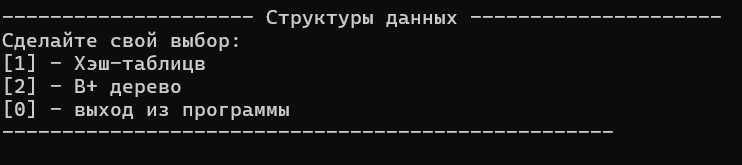
\includegraphics[width=0.9\linewidth]{1}
	\caption{Меню выбора структуры данных}
	\label{fig:1}
\end{figure}

При выборе хеш-таблицы, то есть нажав на клавишу <<1>>, выводится меню для работы с хеш-таблицей (\hyperref[fig:2]{рис.6}).
\begin{figure}[htbp]
	\centering
	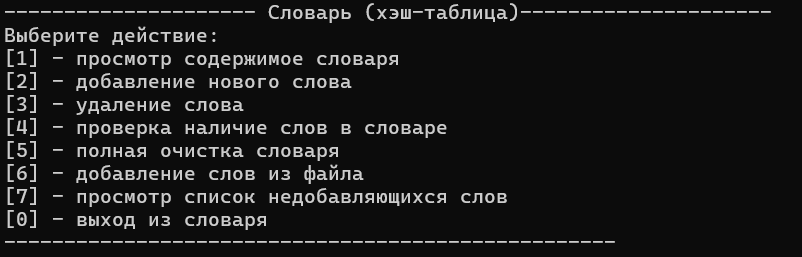
\includegraphics[width=0.9\linewidth]{2}
	\caption{Меню для работы с хеш-таблицей}
	\label{fig:2}
\end{figure}

При нажатии клавиши <<1>>, в самом начале, когда словарь пуст, пользователю будет выведено сообщение о пустом словаре (\hyperref[fig:2.2]{рис.7}).

\begin{figure}[htbp]
	\centering
	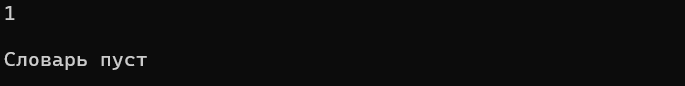
\includegraphics[width=0.9\linewidth]{2.1}
	\caption{Сообщение о пустом словаре}
	\label{fig:2.1}
\end{figure}

\newpage
При нажатии клавиши <<2>>, пользователю предлагается вводить слова, которые он хочет добавить в словарь(\hyperref[fig:3]{рис.8}).

\begin{figure}[htbp]
	\centering
	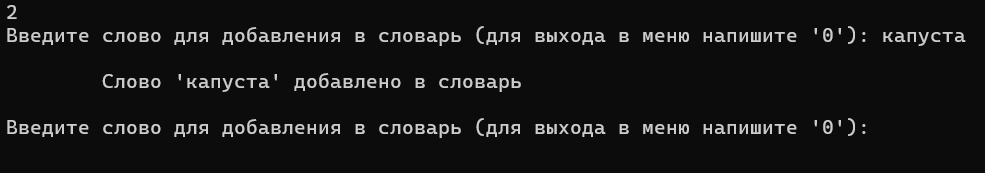
\includegraphics[width=0.9\linewidth]{3}
	\caption{Добавление слов в словарь}
	\label{fig:3}
\end{figure}

При нажатии клавиши <<1>> и наличии в словаре слов, пользователю предлагается вывод в разных форматах: по бакетам и списком (\hyperref[fig:4]{рис.9})

\begin{figure}[htbp]
	\centering
	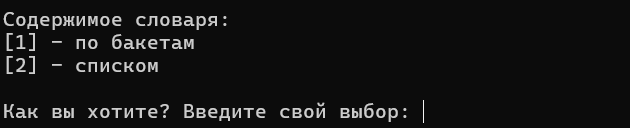
\includegraphics[width=0.9\linewidth]{4}
	\caption{Предложение выбора вывода словаря}
	\label{fig:4}
\end{figure}

При нажатии на <<1>>, слова выводятся по бакетам (\hyperref[fig:5]{рис.10})

\begin{figure}[htbp]
	\centering
	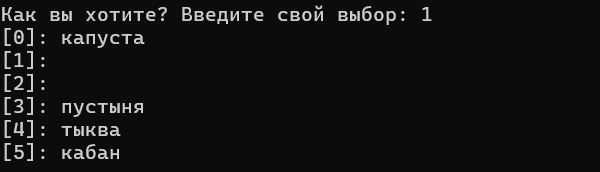
\includegraphics[width=0.9\linewidth]{5}
	\caption{Вывод хеш-таблицы по бакетам}
	\label{fig:5}
\end{figure}

\newpage
Иначе, если нажать <<2>>, слова выведутся одним списком (\hyperref[fig:6]{рис.11})

\begin{figure}[htbp]
	\centering
	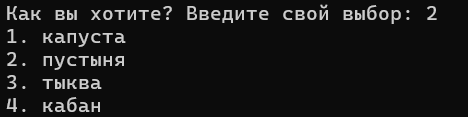
\includegraphics[width=0.9\linewidth]{6}
	\caption{Вывод словаря списком}
	\label{fig:6}
\end{figure}


При нажатии клавиши <<3>>, пользователю предлагается вводить слова, которые он хочет удалить из словаря (\hyperref[fig:7]{рис.12}).

\begin{figure}[htbp]
	\centering
	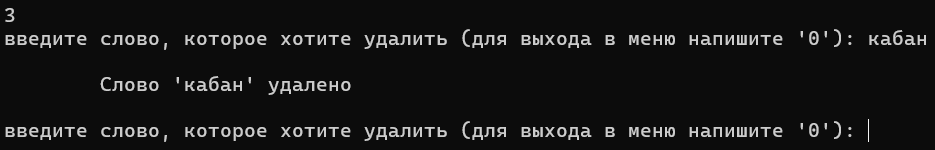
\includegraphics[width=0.9\linewidth]{7}
	\caption{Удаление слова из словаря}
	\label{fig:7}
\end{figure}

При нажатии клавиши <<4>>, пользователю предлагается вводить слова по одному, наличие которых он хочет проверить в словаре (\hyperref[fig:8]{рис.13}).

\begin{figure}[htbp]
	\centering
	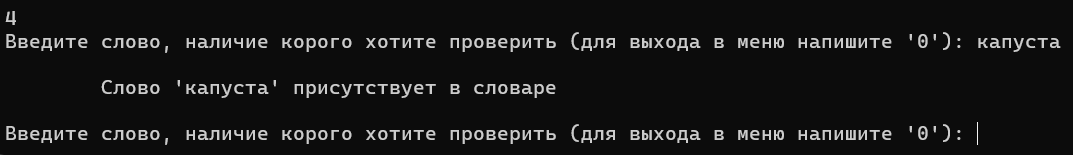
\includegraphics[width=0.9\linewidth]{8}
	\caption{Проверка наличия слова в словаре}
	\label{fig:8}
\end{figure}

\newpage
При нажатии клавиши <<5>> происходит полная очистка словаря (\hyperref[fig:9]{рис.14})

\begin{figure}[htbp]
	\centering
	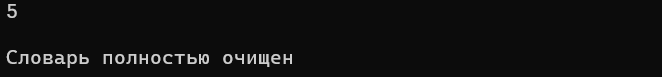
\includegraphics[width=0.9\linewidth]{9}
	\caption{Полная очистка словаря}
	\label{fig:9}
\end{figure}

При нажатии клавиши <<6>> предлагается выбрать файл, из которого будут добавляться слова в хеш-таблицу. Пользователь может выбрать файл из существующих либо выбрать свой файл (\hyperref[fig:10]{рис.15})

\begin{figure}[htbp]
	\centering
	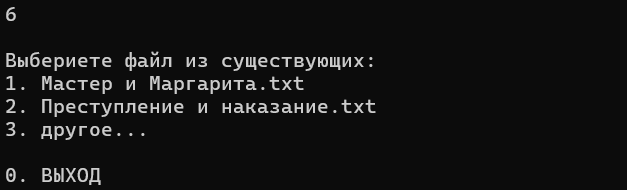
\includegraphics[width=0.9\linewidth]{10}
	\caption{Выбор файла, слова из которого будут добавлены в словарь}
	\label{fig:10}
\end{figure}

Допустим пользователь выбирает файл <<Мастер и Маргарита.txt>>, после выводится сообщение о том, что слова из файла добавлены в словарь (\hyperref[fig:11]{рис.16})

\begin{figure}[htbp]
	\centering
	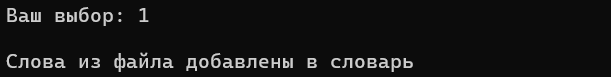
\includegraphics[width=0.9\linewidth]{11}
	\caption{Сообщение о том, что слова из файла добавлены}
	\label{fig:11}
\end{figure}

\newpage
При нажатии клавиши <<7>> пользователю выводится список слов-исключений, которые не будут добавляться в словарь (\hyperref[fig:12]{рис.17})

\begin{figure}[htbp]
	\centering
	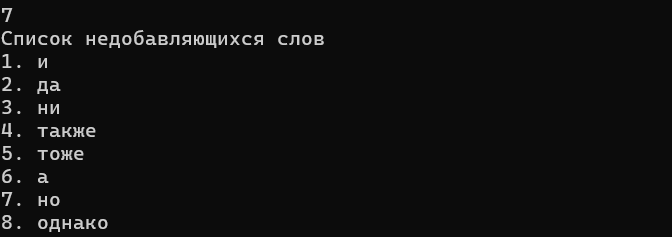
\includegraphics[width=0.9\linewidth]{12}
	\caption{Список слов-исключений}
	\label{fig:12}
\end{figure}

В самом начале при выборе структуры данных, если пользователь нажмет <<2>>, то есть выберет В+-дерево, то выведется меню для работы с В+-деревом  (\hyperref[fig:13]{рис.18})

\begin{figure}[htbp]
	\centering
	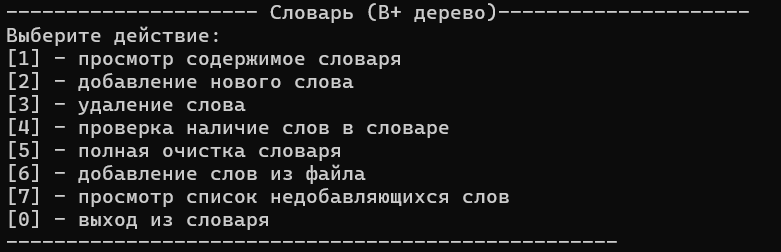
\includegraphics[width=0.9\linewidth]{14}
	\caption{Меню для работы с В+-деревом}
	\label{fig:13}
\end{figure}

При нажатии клавиши <<1>>, в самом начале, когда словарь пуст, пользователю будет выведено сообщение о пустом словаре (\hyperref[fig:14]{рис.19}).

\begin{figure}[htbp]
	\centering
	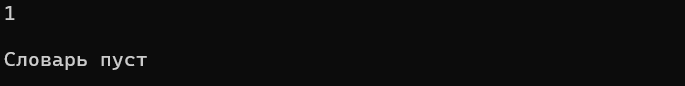
\includegraphics[width=0.9\linewidth]{2.1}
	\caption{Сообщение о пустом словаре}
	\label{fig:14}
\end{figure}

\newpage
При нажатии клавиши <<2>>, пользователю предлагается вводить слова, которые он хочет добавить в словарь(\hyperref[fig:15]{рис.20}).

\begin{figure}[htbp]
	\centering
	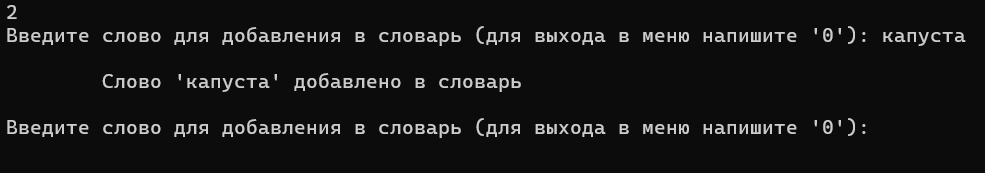
\includegraphics[width=0.9\linewidth]{3}
	\caption{Добавление слов в словарь}
	\label{fig:15}
\end{figure}

При нажатии клавиши <<1>> и наличии в словаре слов, пользователю предлагается вывод в разных форматах: по бакетам и списком (\hyperref[fig:16]{рис.21})

\begin{figure}[htbp]
	\centering
	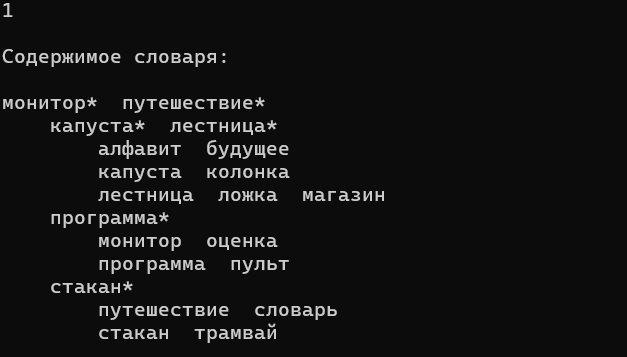
\includegraphics[width=0.9\linewidth]{13}
	\caption{Вывод словаря в виде дерева}
	\label{fig:16}
\end{figure}

При нажатии клавиши <<3>>, пользователю предлагается вводить слова, которые он хочет удалить из словаря (\hyperref[fig:17]{рис.22}).

\begin{figure}[htbp]
	\centering
	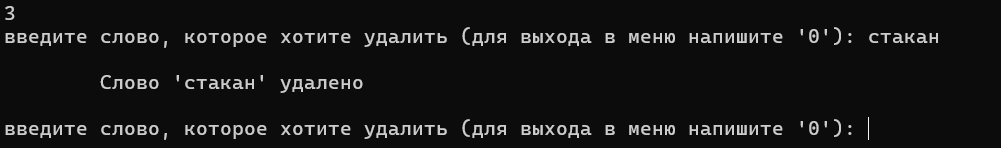
\includegraphics[width=0.9\linewidth]{15}
	\caption{Удаление слова из словаря}
	\label{fig:17}
\end{figure}

\newpage
При нажатии клавиши <<4>>, пользователю предлагается вводить слова по одному, наличие которых он хочет проверить в словаре (\hyperref[fig:18]{рис.23}).

\begin{figure}[htbp]
	\centering
	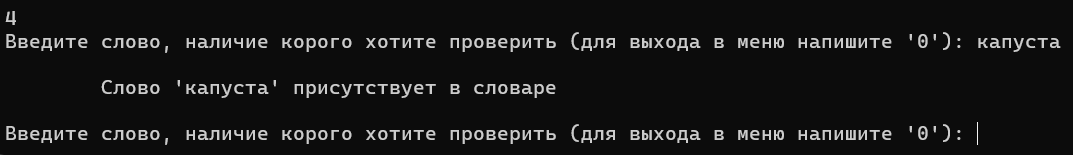
\includegraphics[width=0.9\linewidth]{8}
	\caption{Проверка наличия слова в словаре}
	\label{fig:18}
\end{figure}


При нажатии клавиши <<5>> происходит полная очистка словаря (\hyperref[fig:19]{рис.24})

\begin{figure}[htbp]
	\centering
	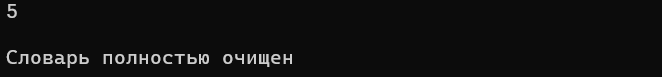
\includegraphics[width=0.9\linewidth]{9}
	\caption{Полная очистка словаря}
	\label{fig:19}
\end{figure}

При нажатии клавиши <<6>> предлагается выбрать файл, из которого будут добавляться слова в В+-дерево. Пользователь может выбрать файл из существующих либо выбрать свой файл (\hyperref[fig:20]{рис.25})

\begin{figure}[htbp]
	\centering
	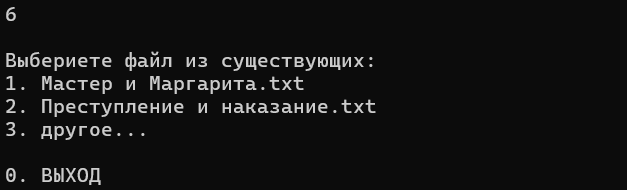
\includegraphics[width=0.9\linewidth]{10}
	\caption{Выбор файла, слова из которого будут добавлены в словарь}
	\label{fig:20}
\end{figure}

\newpage
Допустим пользователь выбирает файл <<Мастер и Маргарита.txt>>, после выводится сообщение о том, что слова из файла добавлены в словарь (\hyperref[fig:21]{рис.26})

\begin{figure}[htbp]
	\centering
	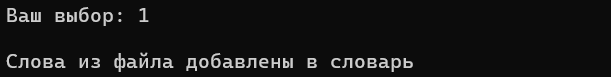
\includegraphics[width=0.9\linewidth]{11}
	\caption{Сообщение о том, что слова из файла добавлены}
	\label{fig:21}
\end{figure}


При нажатии клавиши <<7>> пользователю выводится список слов-исключений, которые не будут добавляться в словарь (\hyperref[fig:22]{рис.27})

\begin{figure}[htbp]
	\centering
	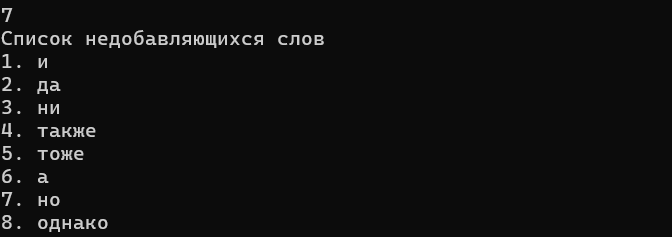
\includegraphics[width=0.9\linewidth]{12}
	\caption{Список слов-исключений}
	\label{fig:22}
\end{figure}

При попытке пользователя ввести некорректное значение, программа выдает об этом сообщение (\hyperref[fig:23]{рис.28})

\begin{figure}[htbp]
	\centering
	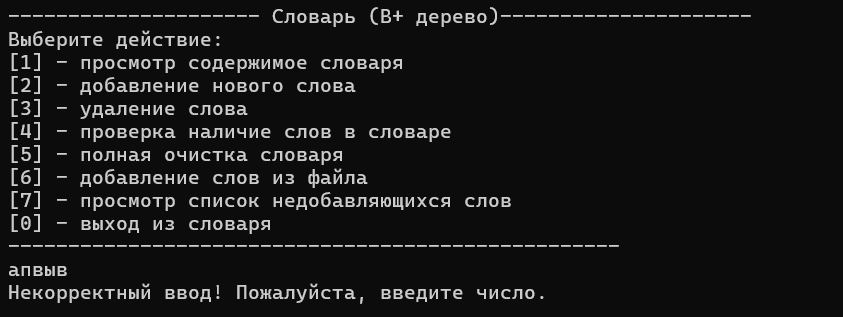
\includegraphics[width=0.9\linewidth]{16}
	\caption{Сообщение о неправильном вводе}
	\label{fig:23}
\end{figure}

\newpage
\section*{Заключение}
\addcontentsline{toc}{section}{Заключение}



В ходе выполнения лабораторной работы был реализован словарь в двух вариантах: хеш-таблицей и B+-деревом. Для каждого из вариантов словаря были реализованы операции: добавления, удаления и поиска слова, полной очистки словаря и добавления слов в словарь из текстового файла. Для разрешения коллизий в хеш-таблице был использован метод цепочек. В хеш-функции хеш слова вычислялся при помощи полинома.\\

Хеш-функция, используемая в хеш-таблице генерирует значения на всем диапазоне переменной int. Чтобы уменьшить количество коллизий была введена переменная - \textbf{коэффициент заполнения}, которая представляет из себя отношение количества элементов в хеш-таблице к общему количеству бакетов. Когда коэффициент заполнения превышает определённый порог (0.75), происходит \textbf{рехеширование} — процесс, при котором создаётся новый массив большего размера с удвоенным количеством бакетов, и все существующие пары из старого массива переносятся в новый, с пересчётом индексов на основе новой хеш-функции. \\

Из достоинств реализованной программы можно назвать наличие функции рехеширования, которая предотвращает появление большого числа коллизий при увеличении количества добавляемых слов, и рассмотрение всех ситуаций при реализации операций добавления и удаления слова из словаря, основанного на B+-дереве.\\

Недостатками реализованной программы можно выделить повторения кода в программе, однотипность хранимых данных, а также то что, В+-дерево в данной программе степени два  \\

В планы на масштабирование программы можно записать следующее:
\begin{enumerate}[label*=\textbullet]
	\item Реализация поиска однокоренных слов в хеш-таблице.
	\item Возможность создания В+-дерева любой, допустимой его свойствам, степени.
	\item Возможность хранения любого типа данных данных структурах.
\end{enumerate}

\newpage
\addcontentsline{toc}{section}{Список использованной литературы}
\begin{thebibliography}{0}
	\bibitem{tema} Секция <<Телематика>>. - Текст: электронный // tema.spbstu.ru : [сайт]. - URL: \href{https://tema.spbstu.ru/tgraph/}{https://tema.spbstu.ru/tgraph/} (дата обращения 12.05.2024).
	\bibitem{novikov}  Новиков, Ф.А. ДИСКРЕТНАЯ МАТЕМАТИКА ДЛЯ ПРОГРАММИСТОВ Ф.А. Новиков. - 3-е издание. - Питер : Питер Пресс, 2009. - 384 с.
\end{thebibliography}

\end{document}